\documentclass[twoside]{book}

% Packages required by doxygen
\usepackage{fixltx2e}
\usepackage{calc}
\usepackage{doxygen}
\usepackage[export]{adjustbox} % also loads graphicx
\usepackage{graphicx}
\usepackage[utf8]{inputenc}
\usepackage{makeidx}
\usepackage{multicol}
\usepackage{multirow}
\PassOptionsToPackage{warn}{textcomp}
\usepackage{textcomp}
\usepackage[nointegrals]{wasysym}
\usepackage[table]{xcolor}

% Font selection
\usepackage[T1]{fontenc}
\usepackage[scaled=.90]{helvet}
\usepackage{courier}
\usepackage{amssymb}
\usepackage{sectsty}
\renewcommand{\familydefault}{\sfdefault}
\allsectionsfont{%
  \fontseries{bc}\selectfont%
  \color{darkgray}%
}
\renewcommand{\DoxyLabelFont}{%
  \fontseries{bc}\selectfont%
  \color{darkgray}%
}
\newcommand{\+}{\discretionary{\mbox{\scriptsize$\hookleftarrow$}}{}{}}

% Page & text layout
\usepackage{geometry}
\geometry{%
  a4paper,%
  top=2.5cm,%
  bottom=2.5cm,%
  left=2.5cm,%
  right=2.5cm%
}
\tolerance=750
\hfuzz=15pt
\hbadness=750
\setlength{\emergencystretch}{15pt}
\setlength{\parindent}{0cm}
\setlength{\parskip}{3ex plus 2ex minus 2ex}
\makeatletter
\renewcommand{\paragraph}{%
  \@startsection{paragraph}{4}{0ex}{-1.0ex}{1.0ex}{%
    \normalfont\normalsize\bfseries\SS@parafont%
  }%
}
\renewcommand{\subparagraph}{%
  \@startsection{subparagraph}{5}{0ex}{-1.0ex}{1.0ex}{%
    \normalfont\normalsize\bfseries\SS@subparafont%
  }%
}
\makeatother

% Headers & footers
\usepackage{fancyhdr}
\pagestyle{fancyplain}
\fancyhead[LE]{\fancyplain{}{\bfseries\thepage}}
\fancyhead[CE]{\fancyplain{}{}}
\fancyhead[RE]{\fancyplain{}{\bfseries\leftmark}}
\fancyhead[LO]{\fancyplain{}{\bfseries\rightmark}}
\fancyhead[CO]{\fancyplain{}{}}
\fancyhead[RO]{\fancyplain{}{\bfseries\thepage}}
\fancyfoot[LE]{\fancyplain{}{}}
\fancyfoot[CE]{\fancyplain{}{}}
\fancyfoot[RE]{\fancyplain{}{\bfseries\scriptsize Generated by Doxygen }}
\fancyfoot[LO]{\fancyplain{}{\bfseries\scriptsize Generated by Doxygen }}
\fancyfoot[CO]{\fancyplain{}{}}
\fancyfoot[RO]{\fancyplain{}{}}
\renewcommand{\footrulewidth}{0.4pt}
\renewcommand{\chaptermark}[1]{%
  \markboth{#1}{}%
}
\renewcommand{\sectionmark}[1]{%
  \markright{\thesection\ #1}%
}

% Indices & bibliography
\usepackage{natbib}
\usepackage[titles]{tocloft}
\setcounter{tocdepth}{3}
\setcounter{secnumdepth}{5}
\makeindex

% Hyperlinks (required, but should be loaded last)
\usepackage{ifpdf}
\ifpdf
  \usepackage[pdftex,pagebackref=true]{hyperref}
\else
  \usepackage[ps2pdf,pagebackref=true]{hyperref}
\fi
\hypersetup{%
  colorlinks=true,%
  linkcolor=blue,%
  citecolor=blue,%
  unicode%
}

% Custom commands
\newcommand{\clearemptydoublepage}{%
  \newpage{\pagestyle{empty}\cleardoublepage}%
}

\usepackage{caption}
\captionsetup{labelsep=space,justification=centering,font={bf},singlelinecheck=off,skip=4pt,position=top}

%===== C O N T E N T S =====

\begin{document}

% Titlepage & ToC
\hypersetup{pageanchor=false,
             bookmarksnumbered=true,
             pdfencoding=unicode
            }
\pagenumbering{roman}
\begin{titlepage}
\vspace*{7cm}
\begin{center}%
{\Large My Project }\\
\vspace*{1cm}
{\large Generated by Doxygen 1.8.11}\\
\end{center}
\end{titlepage}
\clearemptydoublepage
\tableofcontents
\clearemptydoublepage
\pagenumbering{arabic}
\hypersetup{pageanchor=true}

%--- Begin generated contents ---
\chapter{Hierarchical Index}
\section{Class Hierarchy}
This inheritance list is sorted roughly, but not completely, alphabetically\+:\begin{DoxyCompactList}
\item \contentsline{section}{log2hdfs\+:\+:Errmsg\+Handle}{\pageref{classlog2hdfs_1_1ErrmsgHandle}}{}
\item \contentsline{section}{log2hdfs\+:\+:Fp\+Cache}{\pageref{classlog2hdfs_1_1FpCache}}{}
\item \contentsline{section}{log2hdfs\+:\+:Hdfs\+Handle}{\pageref{classlog2hdfs_1_1HdfsHandle}}{}
\begin{DoxyCompactList}
\item \contentsline{section}{log2hdfs\+:\+:Command\+Hdfs\+Handle}{\pageref{classlog2hdfs_1_1CommandHdfsHandle}}{}
\end{DoxyCompactList}
\item \contentsline{section}{log2hdfs\+:\+:Ini\+Config\+Parser}{\pageref{classlog2hdfs_1_1IniConfigParser}}{}
\item \contentsline{section}{log2hdfs\+:\+:Inotify}{\pageref{classlog2hdfs_1_1Inotify}}{}
\item \contentsline{section}{log2hdfs\+:\+:Kafka\+Consume\+Cb}{\pageref{classlog2hdfs_1_1KafkaConsumeCb}}{}
\begin{DoxyCompactList}
\item \contentsline{section}{log2hdfs\+:\+:Consume\+Callback}{\pageref{classlog2hdfs_1_1ConsumeCallback}}{}
\begin{DoxyCompactList}
\item \contentsline{section}{log2hdfs\+:\+:Debug\+Consume\+Callback}{\pageref{classlog2hdfs_1_1DebugConsumeCallback}}{}
\item \contentsline{section}{log2hdfs\+:\+:Report\+Consume\+Callback}{\pageref{classlog2hdfs_1_1ReportConsumeCallback}}{}
\item \contentsline{section}{log2hdfs\+:\+:V6\+Consume\+Callback}{\pageref{classlog2hdfs_1_1V6ConsumeCallback}}{}
\end{DoxyCompactList}
\end{DoxyCompactList}
\item \contentsline{section}{log2hdfs\+:\+:Kafka\+Consumer}{\pageref{classlog2hdfs_1_1KafkaConsumer}}{}
\item \contentsline{section}{log2hdfs\+:\+:Kafka\+Global\+Conf}{\pageref{classlog2hdfs_1_1KafkaGlobalConf}}{}
\item \contentsline{section}{log2hdfs\+:\+:Kafka\+Handle}{\pageref{classlog2hdfs_1_1KafkaHandle}}{}
\item \contentsline{section}{log2hdfs\+:\+:Kafka\+Message}{\pageref{classlog2hdfs_1_1KafkaMessage}}{}
\item \contentsline{section}{log2hdfs\+:\+:Kafka\+Producer}{\pageref{classlog2hdfs_1_1KafkaProducer}}{}
\item \contentsline{section}{log2hdfs\+:\+:Kafka\+Topic}{\pageref{classlog2hdfs_1_1KafkaTopic}}{}
\item \contentsline{section}{log2hdfs\+:\+:Kafka\+Topic\+Conf}{\pageref{classlog2hdfs_1_1KafkaTopicConf}}{}
\item \contentsline{section}{log2hdfs\+:\+:Kafka\+Topic\+Consumer}{\pageref{classlog2hdfs_1_1KafkaTopicConsumer}}{}
\item \contentsline{section}{log2hdfs\+:\+:Kafka\+Topic\+Producer}{\pageref{classlog2hdfs_1_1KafkaTopicProducer}}{}
\item \contentsline{section}{log2hdfs\+:\+:Log\+Format}{\pageref{classlog2hdfs_1_1LogFormat}}{}
\item \contentsline{section}{log2hdfs\+:\+:Message\+Timestamp}{\pageref{classlog2hdfs_1_1MessageTimestamp}}{}
\item \contentsline{section}{log2hdfs\+:\+:Offset\+Table}{\pageref{classlog2hdfs_1_1OffsetTable}}{}
\item \contentsline{section}{log2hdfs\+:\+:Optional$<$ T $>$}{\pageref{classlog2hdfs_1_1Optional}}{}
\item \contentsline{section}{log2hdfs\+:\+:Path\+Format}{\pageref{classlog2hdfs_1_1PathFormat}}{}
\item \contentsline{section}{log2hdfs\+:\+:Produce}{\pageref{classlog2hdfs_1_1Produce}}{}
\item \contentsline{section}{log2hdfs\+:\+:Queue$<$ T $>$}{\pageref{classlog2hdfs_1_1Queue}}{}
\item \contentsline{section}{log2hdfs\+:\+:Section}{\pageref{classlog2hdfs_1_1Section}}{}
\item \contentsline{section}{log2hdfs\+:\+:Topic\+Conf}{\pageref{classlog2hdfs_1_1TopicConf}}{}
\item \contentsline{section}{log2hdfs\+:\+:Topic\+Conf\+Contents}{\pageref{classlog2hdfs_1_1TopicConfContents}}{}
\item \contentsline{section}{log2hdfs\+:\+:Upload}{\pageref{classlog2hdfs_1_1Upload}}{}
\end{DoxyCompactList}

\chapter{Class Index}
\section{Class List}
Here are the classes, structs, unions and interfaces with brief descriptions\+:\begin{DoxyCompactList}
\item\contentsline{section}{\hyperlink{classlog2hdfs_1_1CommandHdfsHandle}{log2hdfs\+::\+Command\+Hdfs\+Handle} }{\pageref{classlog2hdfs_1_1CommandHdfsHandle}}{}
\item\contentsline{section}{\hyperlink{classlog2hdfs_1_1ConsumeCallback}{log2hdfs\+::\+Consume\+Callback} }{\pageref{classlog2hdfs_1_1ConsumeCallback}}{}
\item\contentsline{section}{\hyperlink{classlog2hdfs_1_1DebugConsumeCallback}{log2hdfs\+::\+Debug\+Consume\+Callback} }{\pageref{classlog2hdfs_1_1DebugConsumeCallback}}{}
\item\contentsline{section}{\hyperlink{classlog2hdfs_1_1ErrmsgHandle}{log2hdfs\+::\+Errmsg\+Handle} }{\pageref{classlog2hdfs_1_1ErrmsgHandle}}{}
\item\contentsline{section}{\hyperlink{classlog2hdfs_1_1FpCache}{log2hdfs\+::\+Fp\+Cache} }{\pageref{classlog2hdfs_1_1FpCache}}{}
\item\contentsline{section}{\hyperlink{classlog2hdfs_1_1HdfsHandle}{log2hdfs\+::\+Hdfs\+Handle} }{\pageref{classlog2hdfs_1_1HdfsHandle}}{}
\item\contentsline{section}{\hyperlink{classlog2hdfs_1_1IniConfigParser}{log2hdfs\+::\+Ini\+Config\+Parser} }{\pageref{classlog2hdfs_1_1IniConfigParser}}{}
\item\contentsline{section}{\hyperlink{classlog2hdfs_1_1Inotify}{log2hdfs\+::\+Inotify} }{\pageref{classlog2hdfs_1_1Inotify}}{}
\item\contentsline{section}{\hyperlink{classlog2hdfs_1_1KafkaConsumeCb}{log2hdfs\+::\+Kafka\+Consume\+Cb} }{\pageref{classlog2hdfs_1_1KafkaConsumeCb}}{}
\item\contentsline{section}{\hyperlink{classlog2hdfs_1_1KafkaConsumer}{log2hdfs\+::\+Kafka\+Consumer} }{\pageref{classlog2hdfs_1_1KafkaConsumer}}{}
\item\contentsline{section}{\hyperlink{classlog2hdfs_1_1KafkaGlobalConf}{log2hdfs\+::\+Kafka\+Global\+Conf} }{\pageref{classlog2hdfs_1_1KafkaGlobalConf}}{}
\item\contentsline{section}{\hyperlink{classlog2hdfs_1_1KafkaHandle}{log2hdfs\+::\+Kafka\+Handle} }{\pageref{classlog2hdfs_1_1KafkaHandle}}{}
\item\contentsline{section}{\hyperlink{classlog2hdfs_1_1KafkaMessage}{log2hdfs\+::\+Kafka\+Message} }{\pageref{classlog2hdfs_1_1KafkaMessage}}{}
\item\contentsline{section}{\hyperlink{classlog2hdfs_1_1KafkaProducer}{log2hdfs\+::\+Kafka\+Producer} }{\pageref{classlog2hdfs_1_1KafkaProducer}}{}
\item\contentsline{section}{\hyperlink{classlog2hdfs_1_1KafkaTopic}{log2hdfs\+::\+Kafka\+Topic} }{\pageref{classlog2hdfs_1_1KafkaTopic}}{}
\item\contentsline{section}{\hyperlink{classlog2hdfs_1_1KafkaTopicConf}{log2hdfs\+::\+Kafka\+Topic\+Conf} }{\pageref{classlog2hdfs_1_1KafkaTopicConf}}{}
\item\contentsline{section}{\hyperlink{classlog2hdfs_1_1KafkaTopicConsumer}{log2hdfs\+::\+Kafka\+Topic\+Consumer} }{\pageref{classlog2hdfs_1_1KafkaTopicConsumer}}{}
\item\contentsline{section}{\hyperlink{classlog2hdfs_1_1KafkaTopicProducer}{log2hdfs\+::\+Kafka\+Topic\+Producer} }{\pageref{classlog2hdfs_1_1KafkaTopicProducer}}{}
\item\contentsline{section}{\hyperlink{classlog2hdfs_1_1LogFormat}{log2hdfs\+::\+Log\+Format} }{\pageref{classlog2hdfs_1_1LogFormat}}{}
\item\contentsline{section}{\hyperlink{classlog2hdfs_1_1MessageTimestamp}{log2hdfs\+::\+Message\+Timestamp} }{\pageref{classlog2hdfs_1_1MessageTimestamp}}{}
\item\contentsline{section}{\hyperlink{classlog2hdfs_1_1OffsetTable}{log2hdfs\+::\+Offset\+Table} }{\pageref{classlog2hdfs_1_1OffsetTable}}{}
\item\contentsline{section}{\hyperlink{classlog2hdfs_1_1Optional}{log2hdfs\+::\+Optional$<$ T $>$} }{\pageref{classlog2hdfs_1_1Optional}}{}
\item\contentsline{section}{\hyperlink{classlog2hdfs_1_1PathFormat}{log2hdfs\+::\+Path\+Format} }{\pageref{classlog2hdfs_1_1PathFormat}}{}
\item\contentsline{section}{\hyperlink{classlog2hdfs_1_1Produce}{log2hdfs\+::\+Produce} }{\pageref{classlog2hdfs_1_1Produce}}{}
\item\contentsline{section}{\hyperlink{classlog2hdfs_1_1Queue}{log2hdfs\+::\+Queue$<$ T $>$} }{\pageref{classlog2hdfs_1_1Queue}}{}
\item\contentsline{section}{\hyperlink{classlog2hdfs_1_1ReportConsumeCallback}{log2hdfs\+::\+Report\+Consume\+Callback} }{\pageref{classlog2hdfs_1_1ReportConsumeCallback}}{}
\item\contentsline{section}{\hyperlink{classlog2hdfs_1_1Section}{log2hdfs\+::\+Section} }{\pageref{classlog2hdfs_1_1Section}}{}
\item\contentsline{section}{\hyperlink{classlog2hdfs_1_1TopicConf}{log2hdfs\+::\+Topic\+Conf} }{\pageref{classlog2hdfs_1_1TopicConf}}{}
\item\contentsline{section}{\hyperlink{classlog2hdfs_1_1TopicConfContents}{log2hdfs\+::\+Topic\+Conf\+Contents} }{\pageref{classlog2hdfs_1_1TopicConfContents}}{}
\item\contentsline{section}{\hyperlink{classlog2hdfs_1_1Upload}{log2hdfs\+::\+Upload} }{\pageref{classlog2hdfs_1_1Upload}}{}
\item\contentsline{section}{\hyperlink{classlog2hdfs_1_1V6ConsumeCallback}{log2hdfs\+::\+V6\+Consume\+Callback} }{\pageref{classlog2hdfs_1_1V6ConsumeCallback}}{}
\end{DoxyCompactList}

\chapter{Class Documentation}
\hypertarget{classlog2hdfs_1_1CommandHdfsHandle}{}\section{log2hdfs\+:\+:Command\+Hdfs\+Handle Class Reference}
\label{classlog2hdfs_1_1CommandHdfsHandle}\index{log2hdfs\+::\+Command\+Hdfs\+Handle@{log2hdfs\+::\+Command\+Hdfs\+Handle}}


Inheritance diagram for log2hdfs\+:\+:Command\+Hdfs\+Handle\+:
\nopagebreak
\begin{figure}[H]
\begin{center}
\leavevmode
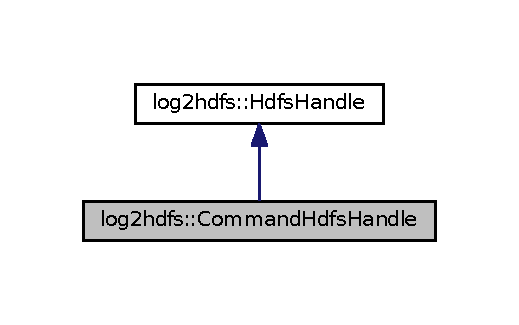
\includegraphics[width=249pt]{classlog2hdfs_1_1CommandHdfsHandle__inherit__graph}
\end{center}
\end{figure}


Collaboration diagram for log2hdfs\+:\+:Command\+Hdfs\+Handle\+:
\nopagebreak
\begin{figure}[H]
\begin{center}
\leavevmode
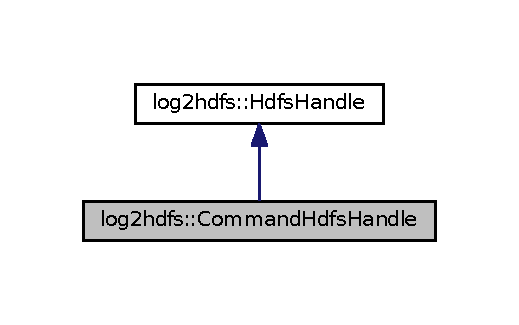
\includegraphics[width=249pt]{classlog2hdfs_1_1CommandHdfsHandle__coll__graph}
\end{center}
\end{figure}
\subsection*{Public Member Functions}
\begin{DoxyCompactItemize}
\item 
{\bfseries Command\+Hdfs\+Handle} (hdfs\+FS fs\+\_\+handle, const std\+::string \&put, const std\+::string \&append, const std\+::string \&lzo\+\_\+index)\hypertarget{classlog2hdfs_1_1CommandHdfsHandle_a6cc703cfb412a5b8d595cb5308d0af73}{}\label{classlog2hdfs_1_1CommandHdfsHandle_a6cc703cfb412a5b8d595cb5308d0af73}

\item 
{\bfseries Command\+Hdfs\+Handle} (const \hyperlink{classlog2hdfs_1_1CommandHdfsHandle}{Command\+Hdfs\+Handle} \&other)=delete\hypertarget{classlog2hdfs_1_1CommandHdfsHandle_a2ebf3179a88faa584f441abd4e009497}{}\label{classlog2hdfs_1_1CommandHdfsHandle_a2ebf3179a88faa584f441abd4e009497}

\item 
\hyperlink{classlog2hdfs_1_1CommandHdfsHandle}{Command\+Hdfs\+Handle} \& {\bfseries operator=} (const \hyperlink{classlog2hdfs_1_1CommandHdfsHandle}{Command\+Hdfs\+Handle} \&other)=delete\hypertarget{classlog2hdfs_1_1CommandHdfsHandle_a22fbe0c5f363e8eba51b1bec46880c41}{}\label{classlog2hdfs_1_1CommandHdfsHandle_a22fbe0c5f363e8eba51b1bec46880c41}

\item 
bool {\bfseries Exists} (const std\+::string \&hdfs\+\_\+path) const \hypertarget{classlog2hdfs_1_1CommandHdfsHandle_aedd6e77ec370ee8d70eb4abd866650e8}{}\label{classlog2hdfs_1_1CommandHdfsHandle_aedd6e77ec370ee8d70eb4abd866650e8}

\item 
bool {\bfseries Put} (const std\+::string \&local\+\_\+path, const std\+::string \&hdfs\+\_\+path) const \hypertarget{classlog2hdfs_1_1CommandHdfsHandle_adf2d5e74962f6fd66a394b4494c32c72}{}\label{classlog2hdfs_1_1CommandHdfsHandle_adf2d5e74962f6fd66a394b4494c32c72}

\item 
bool {\bfseries Append} (const std\+::string \&local\+\_\+path, const std\+::string \&hdfs\+\_\+path) const \hypertarget{classlog2hdfs_1_1CommandHdfsHandle_a39af81a2d01df38e36efcdf2684d601a}{}\label{classlog2hdfs_1_1CommandHdfsHandle_a39af81a2d01df38e36efcdf2684d601a}

\item 
bool {\bfseries Delete} (const std\+::string \&local\+\_\+path) const \hypertarget{classlog2hdfs_1_1CommandHdfsHandle_a0981dd22da8c6dd1561e3180590a4d02}{}\label{classlog2hdfs_1_1CommandHdfsHandle_a0981dd22da8c6dd1561e3180590a4d02}

\item 
bool {\bfseries Create\+Directory} (const std\+::string \&hdfs\+\_\+path) const \hypertarget{classlog2hdfs_1_1CommandHdfsHandle_a92457b8a64a98e1c9df02bb7962b0b71}{}\label{classlog2hdfs_1_1CommandHdfsHandle_a92457b8a64a98e1c9df02bb7962b0b71}

\item 
bool {\bfseries L\+Z\+O\+Index} (const std\+::string \&hdfs\+\_\+path) const \hypertarget{classlog2hdfs_1_1CommandHdfsHandle_a29cc1e78f3c6ad68f3f661f4b397afd9}{}\label{classlog2hdfs_1_1CommandHdfsHandle_a29cc1e78f3c6ad68f3f661f4b397afd9}

\end{DoxyCompactItemize}
\subsection*{Static Public Member Functions}
\begin{DoxyCompactItemize}
\item 
static std\+::shared\+\_\+ptr$<$ \hyperlink{classlog2hdfs_1_1HdfsHandle}{Hdfs\+Handle} $>$ {\bfseries Init} (std\+::shared\+\_\+ptr$<$ \hyperlink{classlog2hdfs_1_1Section}{Section} $>$ section)\hypertarget{classlog2hdfs_1_1CommandHdfsHandle_aa63d52d8d03fde4e0eaaa7beb541024e}{}\label{classlog2hdfs_1_1CommandHdfsHandle_aa63d52d8d03fde4e0eaaa7beb541024e}

\end{DoxyCompactItemize}
\subsection*{Additional Inherited Members}


The documentation for this class was generated from the following files\+:\begin{DoxyCompactItemize}
\item 
src/kafka2hdfs/hdfs\+\_\+handle\+\_\+impl.\+h\item 
src/kafka2hdfs/hdfs\+\_\+handle\+\_\+impl.\+cc\end{DoxyCompactItemize}

\hypertarget{classlog2hdfs_1_1ConsumeCallback}{}\section{log2hdfs\+:\+:Consume\+Callback Class Reference}
\label{classlog2hdfs_1_1ConsumeCallback}\index{log2hdfs\+::\+Consume\+Callback@{log2hdfs\+::\+Consume\+Callback}}


Inheritance diagram for log2hdfs\+:\+:Consume\+Callback\+:
\nopagebreak
\begin{figure}[H]
\begin{center}
\leavevmode
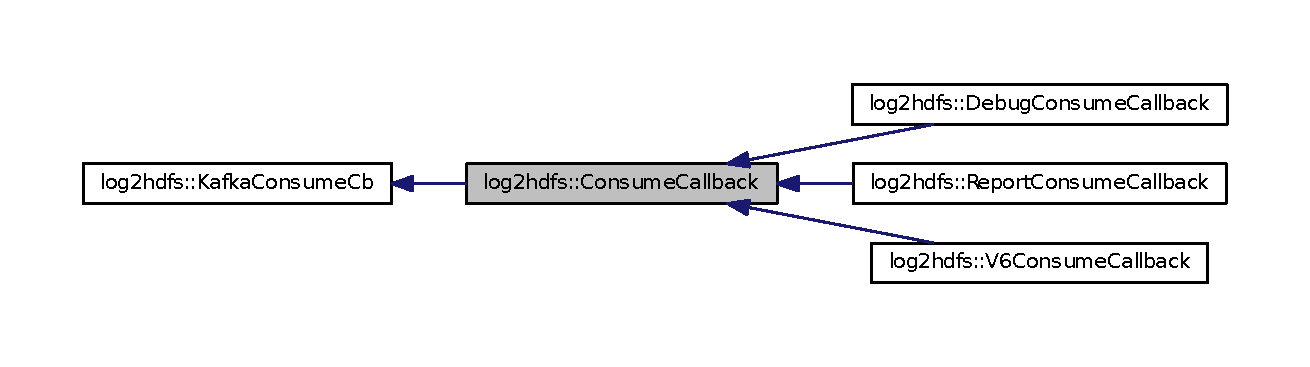
\includegraphics[width=350pt]{classlog2hdfs_1_1ConsumeCallback__inherit__graph}
\end{center}
\end{figure}


Collaboration diagram for log2hdfs\+:\+:Consume\+Callback\+:
\nopagebreak
\begin{figure}[H]
\begin{center}
\leavevmode
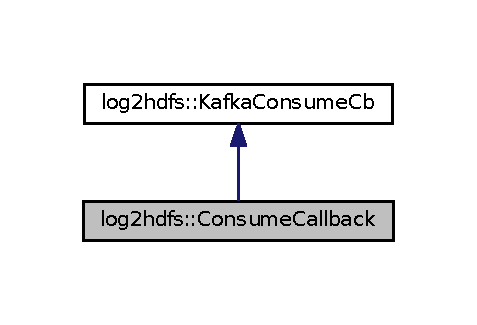
\includegraphics[width=229pt]{classlog2hdfs_1_1ConsumeCallback__coll__graph}
\end{center}
\end{figure}
\subsection*{Public Types}
\begin{DoxyCompactItemize}
\item 
enum {\bfseries Type} \{ \\*
{\bfseries k\+None}, 
{\bfseries k\+V6}, 
{\bfseries k\+Ef}, 
{\bfseries k\+Report}, 
\\*
{\bfseries k\+Debug}
 \}\hypertarget{classlog2hdfs_1_1ConsumeCallback_a039be9af75b6d19dc0221dc869008bc0}{}\label{classlog2hdfs_1_1ConsumeCallback_a039be9af75b6d19dc0221dc869008bc0}

\end{DoxyCompactItemize}
\subsection*{Public Member Functions}
\begin{DoxyCompactItemize}
\item 
{\bfseries Consume\+Callback} (const std\+::string \&dir, std\+::shared\+\_\+ptr$<$ \hyperlink{classlog2hdfs_1_1PathFormat}{Path\+Format} $>$ format, std\+::shared\+\_\+ptr$<$ \hyperlink{classlog2hdfs_1_1FpCache}{Fp\+Cache} $>$ cache)\hypertarget{classlog2hdfs_1_1ConsumeCallback_a695f997b812b87b894283a395d700b6e}{}\label{classlog2hdfs_1_1ConsumeCallback_a695f997b812b87b894283a395d700b6e}

\item 
virtual void {\bfseries Consume} (const \hyperlink{classlog2hdfs_1_1KafkaMessage}{Kafka\+Message} \&msg)=0\hypertarget{classlog2hdfs_1_1ConsumeCallback_a873d0d1a6945dba9730d987907ad85e8}{}\label{classlog2hdfs_1_1ConsumeCallback_a873d0d1a6945dba9730d987907ad85e8}

\end{DoxyCompactItemize}
\subsection*{Static Public Member Functions}
\begin{DoxyCompactItemize}
\item 
static \hyperlink{classlog2hdfs_1_1Optional}{Optional}$<$ Consume\+Callback\+::\+Type $>$ {\bfseries Parse\+Type} (const std\+::string \&type)\hypertarget{classlog2hdfs_1_1ConsumeCallback_ae84b446c67424aad2a4a9bf0bb889cd1}{}\label{classlog2hdfs_1_1ConsumeCallback_ae84b446c67424aad2a4a9bf0bb889cd1}

\item 
static std\+::shared\+\_\+ptr$<$ \hyperlink{classlog2hdfs_1_1KafkaConsumeCb}{Kafka\+Consume\+Cb} $>$ {\bfseries Init} (Consume\+Callback\+::\+Type type, std\+::shared\+\_\+ptr$<$ \hyperlink{classlog2hdfs_1_1TopicConf}{Topic\+Conf} $>$ conf, std\+::shared\+\_\+ptr$<$ \hyperlink{classlog2hdfs_1_1PathFormat}{Path\+Format} $>$ format, std\+::shared\+\_\+ptr$<$ \hyperlink{classlog2hdfs_1_1FpCache}{Fp\+Cache} $>$ cache)\hypertarget{classlog2hdfs_1_1ConsumeCallback_a850e946e425e5c1f8036722a28a68f7f}{}\label{classlog2hdfs_1_1ConsumeCallback_a850e946e425e5c1f8036722a28a68f7f}

\end{DoxyCompactItemize}
\subsection*{Protected Attributes}
\begin{DoxyCompactItemize}
\item 
std\+::string {\bfseries dir\+\_\+}\hypertarget{classlog2hdfs_1_1ConsumeCallback_aaa02dc810d0109654bc3546b9e922273}{}\label{classlog2hdfs_1_1ConsumeCallback_aaa02dc810d0109654bc3546b9e922273}

\item 
std\+::shared\+\_\+ptr$<$ \hyperlink{classlog2hdfs_1_1PathFormat}{Path\+Format} $>$ {\bfseries format\+\_\+}\hypertarget{classlog2hdfs_1_1ConsumeCallback_a777aa5749c2c2ce9d77b997b3bea7373}{}\label{classlog2hdfs_1_1ConsumeCallback_a777aa5749c2c2ce9d77b997b3bea7373}

\item 
std\+::shared\+\_\+ptr$<$ \hyperlink{classlog2hdfs_1_1FpCache}{Fp\+Cache} $>$ {\bfseries cache\+\_\+}\hypertarget{classlog2hdfs_1_1ConsumeCallback_abff2281c0f82754845ff68c23d275284}{}\label{classlog2hdfs_1_1ConsumeCallback_abff2281c0f82754845ff68c23d275284}

\end{DoxyCompactItemize}


The documentation for this class was generated from the following files\+:\begin{DoxyCompactItemize}
\item 
src/kafka2hdfs/consume\+\_\+callback.\+h\item 
src/kafka2hdfs/consume\+\_\+callback.\+cc\end{DoxyCompactItemize}

\hypertarget{classlog2hdfs_1_1DebugConsumeCallback}{}\section{log2hdfs\+:\+:Debug\+Consume\+Callback Class Reference}
\label{classlog2hdfs_1_1DebugConsumeCallback}\index{log2hdfs\+::\+Debug\+Consume\+Callback@{log2hdfs\+::\+Debug\+Consume\+Callback}}


Inheritance diagram for log2hdfs\+:\+:Debug\+Consume\+Callback\+:
\nopagebreak
\begin{figure}[H]
\begin{center}
\leavevmode
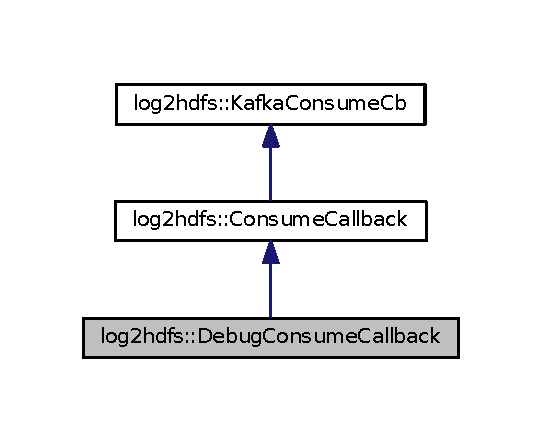
\includegraphics[width=260pt]{classlog2hdfs_1_1DebugConsumeCallback__inherit__graph}
\end{center}
\end{figure}


Collaboration diagram for log2hdfs\+:\+:Debug\+Consume\+Callback\+:
\nopagebreak
\begin{figure}[H]
\begin{center}
\leavevmode
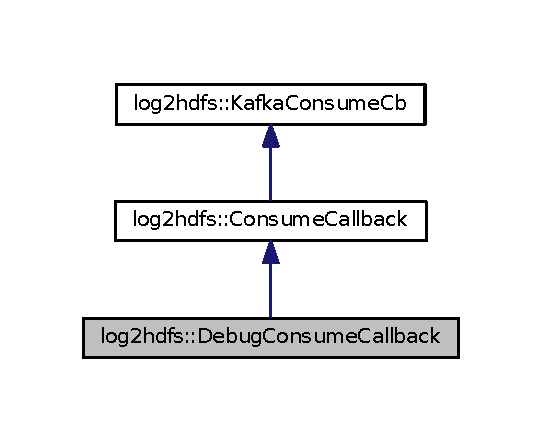
\includegraphics[width=260pt]{classlog2hdfs_1_1DebugConsumeCallback__coll__graph}
\end{center}
\end{figure}
\subsection*{Public Member Functions}
\begin{DoxyCompactItemize}
\item 
{\bfseries Debug\+Consume\+Callback} (const std\+::string \&dir, std\+::shared\+\_\+ptr$<$ \hyperlink{classlog2hdfs_1_1PathFormat}{Path\+Format} $>$ format, std\+::shared\+\_\+ptr$<$ \hyperlink{classlog2hdfs_1_1FpCache}{Fp\+Cache} $>$ cache)\hypertarget{classlog2hdfs_1_1DebugConsumeCallback_a93c8681a3be7473c6ddb33e5366a47b5}{}\label{classlog2hdfs_1_1DebugConsumeCallback_a93c8681a3be7473c6ddb33e5366a47b5}

\item 
{\bfseries Debug\+Consume\+Callback} (const \hyperlink{classlog2hdfs_1_1DebugConsumeCallback}{Debug\+Consume\+Callback} \&other)=delete\hypertarget{classlog2hdfs_1_1DebugConsumeCallback_a907cb23b80e3f5e4cf5a0b903d988e18}{}\label{classlog2hdfs_1_1DebugConsumeCallback_a907cb23b80e3f5e4cf5a0b903d988e18}

\item 
\hyperlink{classlog2hdfs_1_1DebugConsumeCallback}{Debug\+Consume\+Callback} \& {\bfseries operator=} (const \hyperlink{classlog2hdfs_1_1DebugConsumeCallback}{Debug\+Consume\+Callback} \&other)=delete\hypertarget{classlog2hdfs_1_1DebugConsumeCallback_a5222e63ba01c7ebd0b1ff8956d3ab733}{}\label{classlog2hdfs_1_1DebugConsumeCallback_a5222e63ba01c7ebd0b1ff8956d3ab733}

\item 
void {\bfseries Consume} (const \hyperlink{classlog2hdfs_1_1KafkaMessage}{Kafka\+Message} \&msg)\hypertarget{classlog2hdfs_1_1DebugConsumeCallback_aa43ed75073234c2a9d2a1327a2582be7}{}\label{classlog2hdfs_1_1DebugConsumeCallback_aa43ed75073234c2a9d2a1327a2582be7}

\end{DoxyCompactItemize}
\subsection*{Static Public Member Functions}
\begin{DoxyCompactItemize}
\item 
static std\+::shared\+\_\+ptr$<$ \hyperlink{classlog2hdfs_1_1DebugConsumeCallback}{Debug\+Consume\+Callback} $>$ {\bfseries Init} (std\+::shared\+\_\+ptr$<$ \hyperlink{classlog2hdfs_1_1TopicConf}{Topic\+Conf} $>$ conf, std\+::shared\+\_\+ptr$<$ \hyperlink{classlog2hdfs_1_1PathFormat}{Path\+Format} $>$ format, std\+::shared\+\_\+ptr$<$ \hyperlink{classlog2hdfs_1_1FpCache}{Fp\+Cache} $>$ cache)\hypertarget{classlog2hdfs_1_1DebugConsumeCallback_a0002dd402cdf057e28c1189c4c4788fb}{}\label{classlog2hdfs_1_1DebugConsumeCallback_a0002dd402cdf057e28c1189c4c4788fb}

\end{DoxyCompactItemize}
\subsection*{Additional Inherited Members}


The documentation for this class was generated from the following files\+:\begin{DoxyCompactItemize}
\item 
src/kafka2hdfs/consume\+\_\+callback.\+h\item 
src/kafka2hdfs/consume\+\_\+callback.\+cc\end{DoxyCompactItemize}

\hypertarget{classlog2hdfs_1_1ErrmsgHandle}{}\section{log2hdfs\+:\+:Errmsg\+Handle Class Reference}
\label{classlog2hdfs_1_1ErrmsgHandle}\index{log2hdfs\+::\+Errmsg\+Handle@{log2hdfs\+::\+Errmsg\+Handle}}
\subsection*{Public Member Functions}
\begin{DoxyCompactItemize}
\item 
{\bfseries Errmsg\+Handle} (const std\+::string \&dir, int interval, bool remedy, std\+::shared\+\_\+ptr$<$ \hyperlink{classlog2hdfs_1_1FpCache}{Fp\+Cache} $>$ cache, std\+::shared\+\_\+ptr$<$ \hyperlink{classlog2hdfs_1_1Queue}{Queue}$<$ std\+::string $>$$>$ queue)\hypertarget{classlog2hdfs_1_1ErrmsgHandle_afff82775a3da753d8e23ddd1d5199a3e}{}\label{classlog2hdfs_1_1ErrmsgHandle_afff82775a3da753d8e23ddd1d5199a3e}

\item 
{\bfseries Errmsg\+Handle} (const \hyperlink{classlog2hdfs_1_1ErrmsgHandle}{Errmsg\+Handle} \&other)=delete\hypertarget{classlog2hdfs_1_1ErrmsgHandle_aea6310c5bb49db8b43b39cfad6b96743}{}\label{classlog2hdfs_1_1ErrmsgHandle_aea6310c5bb49db8b43b39cfad6b96743}

\item 
\hyperlink{classlog2hdfs_1_1ErrmsgHandle}{Errmsg\+Handle} \& {\bfseries operator=} (const \hyperlink{classlog2hdfs_1_1ErrmsgHandle}{Errmsg\+Handle} \&other)=delete\hypertarget{classlog2hdfs_1_1ErrmsgHandle_a59e51b33003d563924d6646c1d1974ed}{}\label{classlog2hdfs_1_1ErrmsgHandle_a59e51b33003d563924d6646c1d1974ed}

\item 
void {\bfseries Archive\+Msg} (const std\+::string \&topic, const std\+::string \&msg)\hypertarget{classlog2hdfs_1_1ErrmsgHandle_a2c1a0e1df4123d9baf1d8f4af8cd82bf}{}\label{classlog2hdfs_1_1ErrmsgHandle_a2c1a0e1df4123d9baf1d8f4af8cd82bf}

\item 
void {\bfseries Start} ()\hypertarget{classlog2hdfs_1_1ErrmsgHandle_aa729e777f1067d880fa40ede8a629ae8}{}\label{classlog2hdfs_1_1ErrmsgHandle_aa729e777f1067d880fa40ede8a629ae8}

\end{DoxyCompactItemize}
\subsection*{Static Public Member Functions}
\begin{DoxyCompactItemize}
\item 
static std\+::shared\+\_\+ptr$<$ \hyperlink{classlog2hdfs_1_1ErrmsgHandle}{Errmsg\+Handle} $>$ {\bfseries Init} (std\+::shared\+\_\+ptr$<$ \hyperlink{classlog2hdfs_1_1Section}{Section} $>$ section, std\+::shared\+\_\+ptr$<$ \hyperlink{classlog2hdfs_1_1Queue}{Queue}$<$ std\+::string $>$$>$ queue)\hypertarget{classlog2hdfs_1_1ErrmsgHandle_a4e472a2c8e3425249b1ac21e7d324e63}{}\label{classlog2hdfs_1_1ErrmsgHandle_a4e472a2c8e3425249b1ac21e7d324e63}

\end{DoxyCompactItemize}


The documentation for this class was generated from the following files\+:\begin{DoxyCompactItemize}
\item 
src/log2kafka/errmsg\+\_\+handle.\+h\item 
src/log2kafka/errmsg\+\_\+handle.\+cc\end{DoxyCompactItemize}

\hypertarget{classlog2hdfs_1_1FpCache}{}\section{log2hdfs\+:\+:Fp\+Cache Class Reference}
\label{classlog2hdfs_1_1FpCache}\index{log2hdfs\+::\+Fp\+Cache@{log2hdfs\+::\+Fp\+Cache}}


{\ttfamily \#include $<$fp\+\_\+cache.\+h$>$}

\subsection*{Public Types}
\begin{DoxyCompactItemize}
\item 
enum \hyperlink{classlog2hdfs_1_1FpCache_a5a925c5b356be91cf262e5219dafdabe}{Remove\+Result} \{ \hyperlink{classlog2hdfs_1_1FpCache_a5a925c5b356be91cf262e5219dafdabea45c149a2991a004cc2f703028ee8f743}{k\+Invalid\+Key} = -\/2, 
\hyperlink{classlog2hdfs_1_1FpCache_a5a925c5b356be91cf262e5219dafdabea85a0c35bd500ce91be5a049be1e42b82}{k\+Remove\+Failed} = -\/1, 
\hyperlink{classlog2hdfs_1_1FpCache_a5a925c5b356be91cf262e5219dafdabea9fbf001dccee023203b54359e8928193}{k\+Remove\+Ok} = 0
 \}
\end{DoxyCompactItemize}
\subsection*{Public Member Functions}
\begin{DoxyCompactItemize}
\item 
\hyperlink{classlog2hdfs_1_1FpCache_ad897ec187b661d08cacf4daf7847754e}{Fp\+Cache} ()
\item 
\hyperlink{classlog2hdfs_1_1FpCache_a6eb730b44c83f3984a95328a8d31c26e}{$\sim$\+Fp\+Cache} ()
\item 
{\bfseries Fp\+Cache} (const \hyperlink{classlog2hdfs_1_1FpCache}{Fp\+Cache} \&other)=delete\hypertarget{classlog2hdfs_1_1FpCache_ac4ef9c65d099f68cd98416200f703e72}{}\label{classlog2hdfs_1_1FpCache_ac4ef9c65d099f68cd98416200f703e72}

\item 
\hyperlink{classlog2hdfs_1_1FpCache}{Fp\+Cache} \& {\bfseries operator=} (const \hyperlink{classlog2hdfs_1_1FpCache}{Fp\+Cache} \&other)=delete\hypertarget{classlog2hdfs_1_1FpCache_ae476c77e6844928c73205a8816b6ecc4}{}\label{classlog2hdfs_1_1FpCache_ae476c77e6844928c73205a8816b6ecc4}

\item 
std\+::shared\+\_\+ptr$<$ F\+I\+LE $>$ \hyperlink{classlog2hdfs_1_1FpCache_a37b5d20805bd50fcc06b5a3e3c626817}{Get} (const std\+::string \&key)
\item 
std\+::shared\+\_\+ptr$<$ F\+I\+LE $>$ \hyperlink{classlog2hdfs_1_1FpCache_a4685f018669a416f2b495012f42e3eba}{Get} (const std\+::string \&key, const std\+::string \&path)
\item 
\hyperlink{classlog2hdfs_1_1FpCache_a5a925c5b356be91cf262e5219dafdabe}{Fp\+Cache\+::\+Remove\+Result} \hyperlink{classlog2hdfs_1_1FpCache_a5e9a1f0e88c2d8b0b5acfbaee3f8140b}{Remove} (const std\+::string \&key)
\item 
std\+::vector$<$ std\+::string $>$ \hyperlink{classlog2hdfs_1_1FpCache_a420b328e3bb226866f3344d75e13e6e7}{Close\+All} ()
\item 
void {\bfseries Clear} ()\hypertarget{classlog2hdfs_1_1FpCache_ada663f72b8f95401da64156c4f65fdd3}{}\label{classlog2hdfs_1_1FpCache_ada663f72b8f95401da64156c4f65fdd3}

\end{DoxyCompactItemize}
\subsection*{Static Public Member Functions}
\begin{DoxyCompactItemize}
\item 
static std\+::shared\+\_\+ptr$<$ \hyperlink{classlog2hdfs_1_1FpCache}{Fp\+Cache} $>$ {\bfseries Init} ()\hypertarget{classlog2hdfs_1_1FpCache_a01ea7bc476e2cee865d6e425f576e29f}{}\label{classlog2hdfs_1_1FpCache_a01ea7bc476e2cee865d6e425f576e29f}

\end{DoxyCompactItemize}


\subsection{Detailed Description}
Simple thread safe fp cache. 

\subsection{Member Enumeration Documentation}
\index{log2hdfs\+::\+Fp\+Cache@{log2hdfs\+::\+Fp\+Cache}!Remove\+Result@{Remove\+Result}}
\index{Remove\+Result@{Remove\+Result}!log2hdfs\+::\+Fp\+Cache@{log2hdfs\+::\+Fp\+Cache}}
\subsubsection[{\texorpdfstring{Remove\+Result}{RemoveResult}}]{\setlength{\rightskip}{0pt plus 5cm}enum {\bf log2hdfs\+::\+Fp\+Cache\+::\+Remove\+Result}}\hypertarget{classlog2hdfs_1_1FpCache_a5a925c5b356be91cf262e5219dafdabe}{}\label{classlog2hdfs_1_1FpCache_a5a925c5b356be91cf262e5219dafdabe}
\hyperlink{classlog2hdfs_1_1FpCache}{Fp\+Cache} Remove result. \begin{Desc}
\item[Enumerator]\par
\begin{description}
\index{k\+Invalid\+Key@{k\+Invalid\+Key}!log2hdfs\+::\+Fp\+Cache@{log2hdfs\+::\+Fp\+Cache}}\index{log2hdfs\+::\+Fp\+Cache@{log2hdfs\+::\+Fp\+Cache}!k\+Invalid\+Key@{k\+Invalid\+Key}}\item[{\em 
k\+Invalid\+Key\hypertarget{classlog2hdfs_1_1FpCache_a5a925c5b356be91cf262e5219dafdabea45c149a2991a004cc2f703028ee8f743}{}\label{classlog2hdfs_1_1FpCache_a5a925c5b356be91cf262e5219dafdabea45c149a2991a004cc2f703028ee8f743}
}]key was not found. \index{k\+Remove\+Failed@{k\+Remove\+Failed}!log2hdfs\+::\+Fp\+Cache@{log2hdfs\+::\+Fp\+Cache}}\index{log2hdfs\+::\+Fp\+Cache@{log2hdfs\+::\+Fp\+Cache}!k\+Remove\+Failed@{k\+Remove\+Failed}}\item[{\em 
k\+Remove\+Failed\hypertarget{classlog2hdfs_1_1FpCache_a5a925c5b356be91cf262e5219dafdabea85a0c35bd500ce91be5a049be1e42b82}{}\label{classlog2hdfs_1_1FpCache_a5a925c5b356be91cf262e5219dafdabea85a0c35bd500ce91be5a049be1e42b82}
}]remove from map successed but fclose failed. \index{k\+Remove\+Ok@{k\+Remove\+Ok}!log2hdfs\+::\+Fp\+Cache@{log2hdfs\+::\+Fp\+Cache}}\index{log2hdfs\+::\+Fp\+Cache@{log2hdfs\+::\+Fp\+Cache}!k\+Remove\+Ok@{k\+Remove\+Ok}}\item[{\em 
k\+Remove\+Ok\hypertarget{classlog2hdfs_1_1FpCache_a5a925c5b356be91cf262e5219dafdabea9fbf001dccee023203b54359e8928193}{}\label{classlog2hdfs_1_1FpCache_a5a925c5b356be91cf262e5219dafdabea9fbf001dccee023203b54359e8928193}
}]remove and fclose successed. \end{description}
\end{Desc}


\subsection{Constructor \& Destructor Documentation}
\index{log2hdfs\+::\+Fp\+Cache@{log2hdfs\+::\+Fp\+Cache}!Fp\+Cache@{Fp\+Cache}}
\index{Fp\+Cache@{Fp\+Cache}!log2hdfs\+::\+Fp\+Cache@{log2hdfs\+::\+Fp\+Cache}}
\subsubsection[{\texorpdfstring{Fp\+Cache()}{FpCache()}}]{\setlength{\rightskip}{0pt plus 5cm}log2hdfs\+::\+Fp\+Cache\+::\+Fp\+Cache (
\begin{DoxyParamCaption}
{}
\end{DoxyParamCaption}
)\hspace{0.3cm}{\ttfamily [inline]}}\hypertarget{classlog2hdfs_1_1FpCache_ad897ec187b661d08cacf4daf7847754e}{}\label{classlog2hdfs_1_1FpCache_ad897ec187b661d08cacf4daf7847754e}
Constructor.

Init pthread\+\_\+rwlock\+\_\+t. \index{log2hdfs\+::\+Fp\+Cache@{log2hdfs\+::\+Fp\+Cache}!````~Fp\+Cache@{$\sim$\+Fp\+Cache}}
\index{````~Fp\+Cache@{$\sim$\+Fp\+Cache}!log2hdfs\+::\+Fp\+Cache@{log2hdfs\+::\+Fp\+Cache}}
\subsubsection[{\texorpdfstring{$\sim$\+Fp\+Cache()}{~FpCache()}}]{\setlength{\rightskip}{0pt plus 5cm}log2hdfs\+::\+Fp\+Cache\+::$\sim$\+Fp\+Cache (
\begin{DoxyParamCaption}
{}
\end{DoxyParamCaption}
)\hspace{0.3cm}{\ttfamily [inline]}}\hypertarget{classlog2hdfs_1_1FpCache_a6eb730b44c83f3984a95328a8d31c26e}{}\label{classlog2hdfs_1_1FpCache_a6eb730b44c83f3984a95328a8d31c26e}
Destructor.

Clear all F\+I\+L\+E$\ast$ and paths, then destory pthread\+\_\+rwlock\+\_\+t. 

\subsection{Member Function Documentation}
\index{log2hdfs\+::\+Fp\+Cache@{log2hdfs\+::\+Fp\+Cache}!Close\+All@{Close\+All}}
\index{Close\+All@{Close\+All}!log2hdfs\+::\+Fp\+Cache@{log2hdfs\+::\+Fp\+Cache}}
\subsubsection[{\texorpdfstring{Close\+All()}{CloseAll()}}]{\setlength{\rightskip}{0pt plus 5cm}std\+::vector$<$ std\+::string $>$ log2hdfs\+::\+Fp\+Cache\+::\+Close\+All (
\begin{DoxyParamCaption}
{}
\end{DoxyParamCaption}
)}\hypertarget{classlog2hdfs_1_1FpCache_a420b328e3bb226866f3344d75e13e6e7}{}\label{classlog2hdfs_1_1FpCache_a420b328e3bb226866f3344d75e13e6e7}
Erase all fp cache and return cache fp paths. May not thread safe. \index{log2hdfs\+::\+Fp\+Cache@{log2hdfs\+::\+Fp\+Cache}!Get@{Get}}
\index{Get@{Get}!log2hdfs\+::\+Fp\+Cache@{log2hdfs\+::\+Fp\+Cache}}
\subsubsection[{\texorpdfstring{Get(const std\+::string \&key)}{Get(const std::string &key)}}]{\setlength{\rightskip}{0pt plus 5cm}std\+::shared\+\_\+ptr$<$ F\+I\+LE $>$ log2hdfs\+::\+Fp\+Cache\+::\+Get (
\begin{DoxyParamCaption}
\item[{const std\+::string \&}]{key}
\end{DoxyParamCaption}
)}\hypertarget{classlog2hdfs_1_1FpCache_a37b5d20805bd50fcc06b5a3e3c626817}{}\label{classlog2hdfs_1_1FpCache_a37b5d20805bd50fcc06b5a3e3c626817}
Get fp cache from map.


\begin{DoxyParams}{Parameters}
{\em key} & key to match\\
\hline
\end{DoxyParams}
\begin{DoxyReturn}{Returns}
std\+::shared\+\_\+ptr$<$\+F\+I\+L\+E$>$ if key was found; nullptr otherwise. 
\end{DoxyReturn}
\index{log2hdfs\+::\+Fp\+Cache@{log2hdfs\+::\+Fp\+Cache}!Get@{Get}}
\index{Get@{Get}!log2hdfs\+::\+Fp\+Cache@{log2hdfs\+::\+Fp\+Cache}}
\subsubsection[{\texorpdfstring{Get(const std\+::string \&key, const std\+::string \&path)}{Get(const std::string &key, const std::string &path)}}]{\setlength{\rightskip}{0pt plus 5cm}std\+::shared\+\_\+ptr$<$ F\+I\+LE $>$ log2hdfs\+::\+Fp\+Cache\+::\+Get (
\begin{DoxyParamCaption}
\item[{const std\+::string \&}]{key, }
\item[{const std\+::string \&}]{path}
\end{DoxyParamCaption}
)}\hypertarget{classlog2hdfs_1_1FpCache_a4685f018669a416f2b495012f42e3eba}{}\label{classlog2hdfs_1_1FpCache_a4685f018669a416f2b495012f42e3eba}
Get fp cache from map.


\begin{DoxyParams}{Parameters}
{\em key} & key to match \\
\hline
{\em path} & if key not match, path will open\\
\hline
\end{DoxyParams}
\begin{DoxyReturn}{Returns}
std\+::shared\+\_\+ptr$<$\+F\+I\+L\+E$>$ key was found or open(path) successed; nullptr otherwise. 
\end{DoxyReturn}
\index{log2hdfs\+::\+Fp\+Cache@{log2hdfs\+::\+Fp\+Cache}!Remove@{Remove}}
\index{Remove@{Remove}!log2hdfs\+::\+Fp\+Cache@{log2hdfs\+::\+Fp\+Cache}}
\subsubsection[{\texorpdfstring{Remove(const std\+::string \&key)}{Remove(const std::string &key)}}]{\setlength{\rightskip}{0pt plus 5cm}{\bf Fp\+Cache\+::\+Remove\+Result} log2hdfs\+::\+Fp\+Cache\+::\+Remove (
\begin{DoxyParamCaption}
\item[{const std\+::string \&}]{key}
\end{DoxyParamCaption}
)}\hypertarget{classlog2hdfs_1_1FpCache_a5e9a1f0e88c2d8b0b5acfbaee3f8140b}{}\label{classlog2hdfs_1_1FpCache_a5e9a1f0e88c2d8b0b5acfbaee3f8140b}
Remove fp cache from map.


\begin{DoxyParams}{Parameters}
{\em key} & key to math\\
\hline
\end{DoxyParams}
\begin{DoxyReturn}{Returns}
Remove\+Result. 
\end{DoxyReturn}
\begin{DoxySeeAlso}{See also}
\hyperlink{classlog2hdfs_1_1FpCache_a5a925c5b356be91cf262e5219dafdabe}{Remove\+Result} 
\end{DoxySeeAlso}


The documentation for this class was generated from the following files\+:\begin{DoxyCompactItemize}
\item 
src/util/fp\+\_\+cache.\+h\item 
src/util/fp\+\_\+cache.\+cc\end{DoxyCompactItemize}

\hypertarget{classlog2hdfs_1_1HdfsHandle}{}\section{log2hdfs\+:\+:Hdfs\+Handle Class Reference}
\label{classlog2hdfs_1_1HdfsHandle}\index{log2hdfs\+::\+Hdfs\+Handle@{log2hdfs\+::\+Hdfs\+Handle}}


Inheritance diagram for log2hdfs\+:\+:Hdfs\+Handle\+:
\nopagebreak
\begin{figure}[H]
\begin{center}
\leavevmode
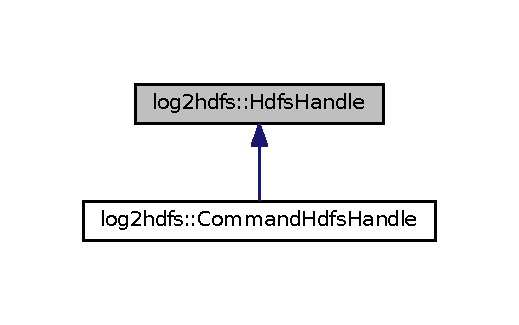
\includegraphics[width=249pt]{classlog2hdfs_1_1HdfsHandle__inherit__graph}
\end{center}
\end{figure}
\subsection*{Public Types}
\begin{DoxyCompactItemize}
\item 
enum {\bfseries Type} \{ {\bfseries k\+Command}, 
{\bfseries k\+Api}
 \}\hypertarget{classlog2hdfs_1_1HdfsHandle_a3540fd28ddf5b29122034b5f11982189}{}\label{classlog2hdfs_1_1HdfsHandle_a3540fd28ddf5b29122034b5f11982189}

\end{DoxyCompactItemize}
\subsection*{Public Member Functions}
\begin{DoxyCompactItemize}
\item 
virtual bool {\bfseries Exists} (const std\+::string \&hdfs\+\_\+path) const =0\hypertarget{classlog2hdfs_1_1HdfsHandle_aa9e0f9d3d7d65f11177fadb02ae87988}{}\label{classlog2hdfs_1_1HdfsHandle_aa9e0f9d3d7d65f11177fadb02ae87988}

\item 
virtual bool {\bfseries Put} (const std\+::string \&local\+\_\+path, const std\+::string \&hdfs\+\_\+path) const =0\hypertarget{classlog2hdfs_1_1HdfsHandle_a9bc69036782f91759d7380f9096d0277}{}\label{classlog2hdfs_1_1HdfsHandle_a9bc69036782f91759d7380f9096d0277}

\item 
virtual bool {\bfseries Append} (const std\+::string \&local\+\_\+path, const std\+::string \&hdfs\+\_\+path) const =0\hypertarget{classlog2hdfs_1_1HdfsHandle_a565087c82689cadad87d886ffabc99d2}{}\label{classlog2hdfs_1_1HdfsHandle_a565087c82689cadad87d886ffabc99d2}

\item 
virtual bool {\bfseries Delete} (const std\+::string \&hdfs\+\_\+path) const =0\hypertarget{classlog2hdfs_1_1HdfsHandle_aa8bd7cbe09e716420b55cc1b0948956e}{}\label{classlog2hdfs_1_1HdfsHandle_aa8bd7cbe09e716420b55cc1b0948956e}

\item 
virtual bool {\bfseries Create\+Directory} (const std\+::string \&hdfs\+\_\+path) const =0\hypertarget{classlog2hdfs_1_1HdfsHandle_aee932d7458c2afebcda1a5a249299859}{}\label{classlog2hdfs_1_1HdfsHandle_aee932d7458c2afebcda1a5a249299859}

\item 
virtual bool {\bfseries L\+Z\+O\+Index} (const std\+::string \&hdfs\+\_\+path) const =0\hypertarget{classlog2hdfs_1_1HdfsHandle_a3cff55576ac5171ed844ccb17ccb436e}{}\label{classlog2hdfs_1_1HdfsHandle_a3cff55576ac5171ed844ccb17ccb436e}

\end{DoxyCompactItemize}
\subsection*{Static Public Member Functions}
\begin{DoxyCompactItemize}
\item 
static std\+::shared\+\_\+ptr$<$ \hyperlink{classlog2hdfs_1_1HdfsHandle}{Hdfs\+Handle} $>$ {\bfseries Init} (std\+::shared\+\_\+ptr$<$ \hyperlink{classlog2hdfs_1_1Section}{Section} $>$ section)\hypertarget{classlog2hdfs_1_1HdfsHandle_a3de62a0bfaf781ea4507bef265694ba4}{}\label{classlog2hdfs_1_1HdfsHandle_a3de62a0bfaf781ea4507bef265694ba4}

\end{DoxyCompactItemize}


The documentation for this class was generated from the following files\+:\begin{DoxyCompactItemize}
\item 
src/kafka2hdfs/hdfs\+\_\+handle.\+h\item 
src/kafka2hdfs/hdfs\+\_\+handle\+\_\+impl.\+cc\end{DoxyCompactItemize}

\hypertarget{classlog2hdfs_1_1IniConfigParser}{}\section{log2hdfs\+:\+:Ini\+Config\+Parser Class Reference}
\label{classlog2hdfs_1_1IniConfigParser}\index{log2hdfs\+::\+Ini\+Config\+Parser@{log2hdfs\+::\+Ini\+Config\+Parser}}
\subsection*{Public Types}
\begin{DoxyCompactItemize}
\item 
typedef std\+::unordered\+\_\+map$<$ std\+::string, std\+::shared\+\_\+ptr$<$ \hyperlink{classlog2hdfs_1_1Section}{Section} $>$ $>$\+::iterator {\bfseries iterator}\hypertarget{classlog2hdfs_1_1IniConfigParser_aa9fda92b7dac941dd1b5ebb92eba684f}{}\label{classlog2hdfs_1_1IniConfigParser_aa9fda92b7dac941dd1b5ebb92eba684f}

\item 
typedef std\+::unordered\+\_\+map$<$ std\+::string, std\+::shared\+\_\+ptr$<$ \hyperlink{classlog2hdfs_1_1Section}{Section} $>$ $>$\+::const\+\_\+iterator {\bfseries const\+\_\+iterator}\hypertarget{classlog2hdfs_1_1IniConfigParser_ab4bb963379b16f07f5704ed0df15ec95}{}\label{classlog2hdfs_1_1IniConfigParser_ab4bb963379b16f07f5704ed0df15ec95}

\end{DoxyCompactItemize}
\subsection*{Public Member Functions}
\begin{DoxyCompactItemize}
\item 
{\bfseries Ini\+Config\+Parser} (const \hyperlink{classlog2hdfs_1_1IniConfigParser}{Ini\+Config\+Parser} \&other)\hypertarget{classlog2hdfs_1_1IniConfigParser_a9d4ef61cd9269503552c45b3290e21de}{}\label{classlog2hdfs_1_1IniConfigParser_a9d4ef61cd9269503552c45b3290e21de}

\item 
{\bfseries Ini\+Config\+Parser} (\hyperlink{classlog2hdfs_1_1IniConfigParser}{Ini\+Config\+Parser} \&\&other)\hypertarget{classlog2hdfs_1_1IniConfigParser_acb529019833028c7c2f3c70793e520a4}{}\label{classlog2hdfs_1_1IniConfigParser_acb529019833028c7c2f3c70793e520a4}

\item 
\hyperlink{classlog2hdfs_1_1IniConfigParser}{Ini\+Config\+Parser} \& {\bfseries operator=} (const \hyperlink{classlog2hdfs_1_1IniConfigParser}{Ini\+Config\+Parser} \&other)\hypertarget{classlog2hdfs_1_1IniConfigParser_ab09d0f609f4c65484547d0230881b606}{}\label{classlog2hdfs_1_1IniConfigParser_ab09d0f609f4c65484547d0230881b606}

\item 
\hyperlink{classlog2hdfs_1_1IniConfigParser}{Ini\+Config\+Parser} \& {\bfseries operator=} (const \hyperlink{classlog2hdfs_1_1IniConfigParser}{Ini\+Config\+Parser} \&\&other)\hypertarget{classlog2hdfs_1_1IniConfigParser_ad8d28b244d3270b5cc29b8fcf72393cf}{}\label{classlog2hdfs_1_1IniConfigParser_ad8d28b244d3270b5cc29b8fcf72393cf}

\item 
bool {\bfseries Has\+Section} (const std\+::string \&section) const \hypertarget{classlog2hdfs_1_1IniConfigParser_ad8353947ca41522c7693d46a49100361}{}\label{classlog2hdfs_1_1IniConfigParser_ad8353947ca41522c7693d46a49100361}

\item 
bool {\bfseries Add\+Section} (const std\+::string \&section)\hypertarget{classlog2hdfs_1_1IniConfigParser_a4a61b4b5843622039e36bb0947a33344}{}\label{classlog2hdfs_1_1IniConfigParser_a4a61b4b5843622039e36bb0947a33344}

\item 
bool {\bfseries Remove\+Section} (const std\+::string \&section)\hypertarget{classlog2hdfs_1_1IniConfigParser_a32b3293011b19876351a27653925cf8c}{}\label{classlog2hdfs_1_1IniConfigParser_a32b3293011b19876351a27653925cf8c}

\item 
std\+::shared\+\_\+ptr$<$ \hyperlink{classlog2hdfs_1_1Section}{Section} $>$ {\bfseries Get\+Section} (const std\+::string \&section)\hypertarget{classlog2hdfs_1_1IniConfigParser_aeee13031c12b4d3fdf857acd3347f0d8}{}\label{classlog2hdfs_1_1IniConfigParser_aeee13031c12b4d3fdf857acd3347f0d8}

\item 
bool {\bfseries Has\+Option} (const std\+::string \&section, const std\+::string \&option) const \hypertarget{classlog2hdfs_1_1IniConfigParser_a280e18ede56472f6325d00fe34271a6c}{}\label{classlog2hdfs_1_1IniConfigParser_a280e18ede56472f6325d00fe34271a6c}

\item 
bool {\bfseries Remove\+Option} (const std\+::string \&section, const std\+::string \&option)\hypertarget{classlog2hdfs_1_1IniConfigParser_abf3278e73c150db0fb091b7d9ed15da0}{}\label{classlog2hdfs_1_1IniConfigParser_abf3278e73c150db0fb091b7d9ed15da0}

\item 
\hyperlink{classlog2hdfs_1_1Optional}{Optional}$<$ std\+::string $>$ {\bfseries Get} (const std\+::string \&section, const std\+::string \&option) const \hypertarget{classlog2hdfs_1_1IniConfigParser_a0930726f5c508fd9684c0758e02bc1aa}{}\label{classlog2hdfs_1_1IniConfigParser_a0930726f5c508fd9684c0758e02bc1aa}

\item 
std\+::string {\bfseries Get} (const std\+::string \&section, const std\+::string \&option, const std\+::string \&default\+\_\+value) const \hypertarget{classlog2hdfs_1_1IniConfigParser_af3e496884b1f0c5820c941b8d21b6e9d}{}\label{classlog2hdfs_1_1IniConfigParser_af3e496884b1f0c5820c941b8d21b6e9d}

\item 
bool {\bfseries Set} (const std\+::string \&section, const std\+::string \&option, const std\+::string \&value)\hypertarget{classlog2hdfs_1_1IniConfigParser_a1b8deba703a74c1539295760a7e794ee}{}\label{classlog2hdfs_1_1IniConfigParser_a1b8deba703a74c1539295760a7e794ee}

\item 
Ini\+Config\+Parser\+::iterator {\bfseries Begin} ()\hypertarget{classlog2hdfs_1_1IniConfigParser_a514a95d5e7f8f3d1119d446e0a5bc39d}{}\label{classlog2hdfs_1_1IniConfigParser_a514a95d5e7f8f3d1119d446e0a5bc39d}

\item 
Ini\+Config\+Parser\+::iterator {\bfseries End} ()\hypertarget{classlog2hdfs_1_1IniConfigParser_a3bbc39cd2701e0411065328285faef37}{}\label{classlog2hdfs_1_1IniConfigParser_a3bbc39cd2701e0411065328285faef37}

\item 
Ini\+Config\+Parser\+::const\+\_\+iterator {\bfseries Begin} () const \hypertarget{classlog2hdfs_1_1IniConfigParser_ab1c7cf51560f0e4b7172defa1900b948}{}\label{classlog2hdfs_1_1IniConfigParser_ab1c7cf51560f0e4b7172defa1900b948}

\item 
Ini\+Config\+Parser\+::const\+\_\+iterator {\bfseries End} () const \hypertarget{classlog2hdfs_1_1IniConfigParser_a5ab4ebd42acd0993db74c55d60468ae7}{}\label{classlog2hdfs_1_1IniConfigParser_a5ab4ebd42acd0993db74c55d60468ae7}

\item 
bool {\bfseries Empty} () const \hypertarget{classlog2hdfs_1_1IniConfigParser_a489246260e96bcd7b714d7873b298a6a}{}\label{classlog2hdfs_1_1IniConfigParser_a489246260e96bcd7b714d7873b298a6a}

\item 
void {\bfseries Clear} ()\hypertarget{classlog2hdfs_1_1IniConfigParser_a3a322d4842c048c51e9e31ec817ac29c}{}\label{classlog2hdfs_1_1IniConfigParser_a3a322d4842c048c51e9e31ec817ac29c}

\item 
bool {\bfseries Read} (const std\+::string \&filepath)\hypertarget{classlog2hdfs_1_1IniConfigParser_a3863dfedd40a884fa7b7dc7db718e88d}{}\label{classlog2hdfs_1_1IniConfigParser_a3863dfedd40a884fa7b7dc7db718e88d}

\item 
bool {\bfseries Write} (const std\+::string \&filepath) const \hypertarget{classlog2hdfs_1_1IniConfigParser_a0a145c323b3fff62e405645c88f78b6c}{}\label{classlog2hdfs_1_1IniConfigParser_a0a145c323b3fff62e405645c88f78b6c}

\end{DoxyCompactItemize}
\subsection*{Static Public Member Functions}
\begin{DoxyCompactItemize}
\item 
static std\+::shared\+\_\+ptr$<$ \hyperlink{classlog2hdfs_1_1IniConfigParser}{Ini\+Config\+Parser} $>$ {\bfseries Init} ()\hypertarget{classlog2hdfs_1_1IniConfigParser_a78747e0d07c0789a29941b4e284ac6b8}{}\label{classlog2hdfs_1_1IniConfigParser_a78747e0d07c0789a29941b4e284ac6b8}

\end{DoxyCompactItemize}


The documentation for this class was generated from the following files\+:\begin{DoxyCompactItemize}
\item 
src/util/configparser.\+h\item 
src/util/configparser.\+cc\end{DoxyCompactItemize}

\hypertarget{classlog2hdfs_1_1Inotify}{}\section{log2hdfs\+:\+:Inotify Class Reference}
\label{classlog2hdfs_1_1Inotify}\index{log2hdfs\+::\+Inotify@{log2hdfs\+::\+Inotify}}
\subsection*{Public Member Functions}
\begin{DoxyCompactItemize}
\item 
{\bfseries Inotify} (int inot\+\_\+fd, std\+::shared\+\_\+ptr$<$ \hyperlink{classlog2hdfs_1_1Queue}{Queue}$<$ std\+::string $>$$>$ queue, std\+::shared\+\_\+ptr$<$ \hyperlink{classlog2hdfs_1_1OffsetTable}{Offset\+Table} $>$ table)\hypertarget{classlog2hdfs_1_1Inotify_ad34071284752c9a410b22acf8d3a3edd}{}\label{classlog2hdfs_1_1Inotify_ad34071284752c9a410b22acf8d3a3edd}

\item 
bool {\bfseries Add\+Watch\+Topic} (std\+::shared\+\_\+ptr$<$ \hyperlink{classlog2hdfs_1_1TopicConf}{Topic\+Conf} $>$ conf)\hypertarget{classlog2hdfs_1_1Inotify_a0d316fc6484ae37b0b12873e606ca4ab}{}\label{classlog2hdfs_1_1Inotify_a0d316fc6484ae37b0b12873e606ca4ab}

\item 
bool {\bfseries Remove\+Watch\+Topic} (const std\+::string \&topic)\hypertarget{classlog2hdfs_1_1Inotify_a4480eae9ea09fc9f195f2a08cb8ccd99}{}\label{classlog2hdfs_1_1Inotify_a4480eae9ea09fc9f195f2a08cb8ccd99}

\item 
bool {\bfseries Add\+Watch\+Path} (const std\+::string \&topic, const std\+::string \&path, time\+\_\+t remedy)\hypertarget{classlog2hdfs_1_1Inotify_a4e895da7dc26306f631e821beb4840c7}{}\label{classlog2hdfs_1_1Inotify_a4e895da7dc26306f631e821beb4840c7}

\item 
void {\bfseries Start} ()\hypertarget{classlog2hdfs_1_1Inotify_a7cefaa00dd6a0df4d0d2e43dbaccc453}{}\label{classlog2hdfs_1_1Inotify_a7cefaa00dd6a0df4d0d2e43dbaccc453}

\end{DoxyCompactItemize}
\subsection*{Static Public Member Functions}
\begin{DoxyCompactItemize}
\item 
static std\+::unique\+\_\+ptr$<$ \hyperlink{classlog2hdfs_1_1Inotify}{Inotify} $>$ {\bfseries Init} (std\+::shared\+\_\+ptr$<$ \hyperlink{classlog2hdfs_1_1Queue}{Queue}$<$ std\+::string $>$$>$ queue, std\+::shared\+\_\+ptr$<$ \hyperlink{classlog2hdfs_1_1OffsetTable}{Offset\+Table} $>$ table)\hypertarget{classlog2hdfs_1_1Inotify_a0b7430c48efb49c67554003ae0cd313a}{}\label{classlog2hdfs_1_1Inotify_a0b7430c48efb49c67554003ae0cd313a}

\end{DoxyCompactItemize}


The documentation for this class was generated from the following files\+:\begin{DoxyCompactItemize}
\item 
src/log2kafka/inotify.\+h\item 
src/log2kafka/inotify.\+cc\end{DoxyCompactItemize}

\hypertarget{classlog2hdfs_1_1KafkaConsumeCb}{}\section{log2hdfs\+:\+:Kafka\+Consume\+Cb Class Reference}
\label{classlog2hdfs_1_1KafkaConsumeCb}\index{log2hdfs\+::\+Kafka\+Consume\+Cb@{log2hdfs\+::\+Kafka\+Consume\+Cb}}


Inheritance diagram for log2hdfs\+:\+:Kafka\+Consume\+Cb\+:
\nopagebreak
\begin{figure}[H]
\begin{center}
\leavevmode
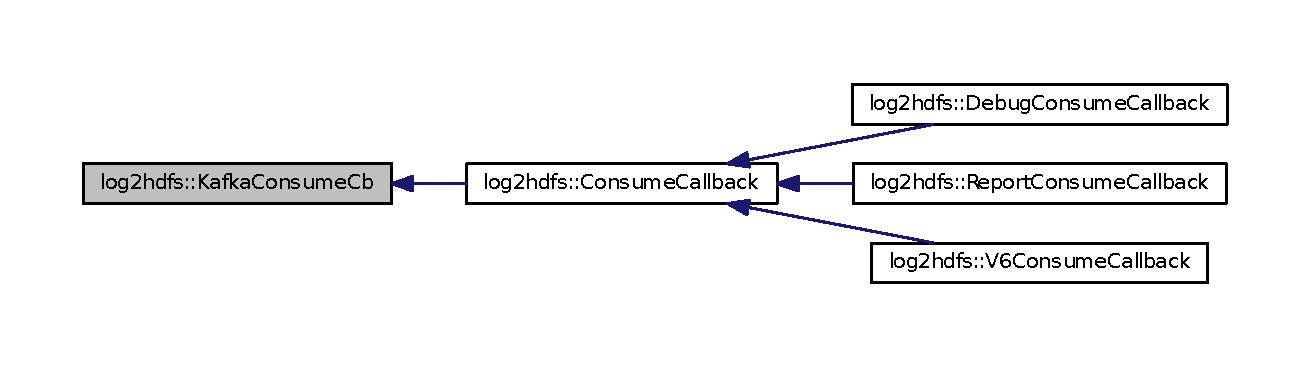
\includegraphics[width=350pt]{classlog2hdfs_1_1KafkaConsumeCb__inherit__graph}
\end{center}
\end{figure}
\subsection*{Public Member Functions}
\begin{DoxyCompactItemize}
\item 
virtual void {\bfseries Consume} (const \hyperlink{classlog2hdfs_1_1KafkaMessage}{Kafka\+Message} \&msg)=0\hypertarget{classlog2hdfs_1_1KafkaConsumeCb_a4eb2387a0688e2db2167b0cba341cafa}{}\label{classlog2hdfs_1_1KafkaConsumeCb_a4eb2387a0688e2db2167b0cba341cafa}

\end{DoxyCompactItemize}


The documentation for this class was generated from the following file\+:\begin{DoxyCompactItemize}
\item 
src/kafka/kafka\+\_\+topic\+\_\+consumer.\+h\end{DoxyCompactItemize}

\hypertarget{classlog2hdfs_1_1KafkaConsumer}{}\section{log2hdfs\+:\+:Kafka\+Consumer Class Reference}
\label{classlog2hdfs_1_1KafkaConsumer}\index{log2hdfs\+::\+Kafka\+Consumer@{log2hdfs\+::\+Kafka\+Consumer}}
\subsection*{Public Member Functions}
\begin{DoxyCompactItemize}
\item 
{\bfseries Kafka\+Consumer} (std\+::shared\+\_\+ptr$<$ \hyperlink{classlog2hdfs_1_1KafkaHandle}{Kafka\+Handle} $>$ handle)\hypertarget{classlog2hdfs_1_1KafkaConsumer_af4e1f7a77ee5c7b713aae6cc7722ef20}{}\label{classlog2hdfs_1_1KafkaConsumer_af4e1f7a77ee5c7b713aae6cc7722ef20}

\item 
{\bfseries Kafka\+Consumer} (const \hyperlink{classlog2hdfs_1_1KafkaConsumer}{Kafka\+Consumer} \&other)=delete\hypertarget{classlog2hdfs_1_1KafkaConsumer_aa71f0b187f30908fd930f0103aaadb7a}{}\label{classlog2hdfs_1_1KafkaConsumer_aa71f0b187f30908fd930f0103aaadb7a}

\item 
\hyperlink{classlog2hdfs_1_1KafkaConsumer}{Kafka\+Consumer} \& {\bfseries operator=} (const \hyperlink{classlog2hdfs_1_1KafkaConsumer}{Kafka\+Consumer} \&other)=delete\hypertarget{classlog2hdfs_1_1KafkaConsumer_a21dc6d1b3dd655ceac6d31b389dca272}{}\label{classlog2hdfs_1_1KafkaConsumer_a21dc6d1b3dd655ceac6d31b389dca272}

\item 
const std\+::string {\bfseries Name} () const \hypertarget{classlog2hdfs_1_1KafkaConsumer_a6483ec9c17558953d4beae9fafeb9039}{}\label{classlog2hdfs_1_1KafkaConsumer_a6483ec9c17558953d4beae9fafeb9039}

\item 
const std\+::string {\bfseries Member\+Id} () const \hypertarget{classlog2hdfs_1_1KafkaConsumer_a43b5de3d00314b6ae52be31ef5ed7a00}{}\label{classlog2hdfs_1_1KafkaConsumer_a43b5de3d00314b6ae52be31ef5ed7a00}

\item 
std\+::shared\+\_\+ptr$<$ \hyperlink{classlog2hdfs_1_1KafkaTopicConsumer}{Kafka\+Topic\+Consumer} $>$ {\bfseries Create\+Topic\+Consumer} (const std\+::string \&topic, \hyperlink{classlog2hdfs_1_1KafkaTopicConf}{Kafka\+Topic\+Conf} $\ast$conf, const std\+::vector$<$ int32\+\_\+t $>$ \&partitions, const std\+::vector$<$ int64\+\_\+t $>$ \&offsets, std\+::shared\+\_\+ptr$<$ \hyperlink{classlog2hdfs_1_1KafkaConsumeCb}{Kafka\+Consume\+Cb} $>$ cb, std\+::string $\ast$errstr)\hypertarget{classlog2hdfs_1_1KafkaConsumer_aeffdb734cf330462b9ba3c2fe4d78ce9}{}\label{classlog2hdfs_1_1KafkaConsumer_aeffdb734cf330462b9ba3c2fe4d78ce9}

\item 
void {\bfseries Start\+All\+Topic} ()\hypertarget{classlog2hdfs_1_1KafkaConsumer_a4c5323c2b8aa7879151f937aa278865c}{}\label{classlog2hdfs_1_1KafkaConsumer_a4c5323c2b8aa7879151f937aa278865c}

\item 
void {\bfseries Stop\+All\+Topic} ()\hypertarget{classlog2hdfs_1_1KafkaConsumer_a8c6fa096dff438222fe5faa8e6534a36}{}\label{classlog2hdfs_1_1KafkaConsumer_a8c6fa096dff438222fe5faa8e6534a36}

\item 
bool {\bfseries Start\+Topic} (const std\+::string \&topic)\hypertarget{classlog2hdfs_1_1KafkaConsumer_a64aaf4d6b6c9b80475a36b7033fbf681}{}\label{classlog2hdfs_1_1KafkaConsumer_a64aaf4d6b6c9b80475a36b7033fbf681}

\item 
bool {\bfseries Stop\+Topic} (const std\+::string \&topic)\hypertarget{classlog2hdfs_1_1KafkaConsumer_a193777bd396d2b3adf4d8f591076b79d}{}\label{classlog2hdfs_1_1KafkaConsumer_a193777bd396d2b3adf4d8f591076b79d}

\end{DoxyCompactItemize}
\subsection*{Static Public Member Functions}
\begin{DoxyCompactItemize}
\item 
static std\+::shared\+\_\+ptr$<$ \hyperlink{classlog2hdfs_1_1KafkaConsumer}{Kafka\+Consumer} $>$ {\bfseries Init} (\hyperlink{classlog2hdfs_1_1KafkaGlobalConf}{Kafka\+Global\+Conf} $\ast$conf, std\+::string $\ast$errstr)\hypertarget{classlog2hdfs_1_1KafkaConsumer_a29cabdb7effeecfa881b0cf90fe84ae1}{}\label{classlog2hdfs_1_1KafkaConsumer_a29cabdb7effeecfa881b0cf90fe84ae1}

\end{DoxyCompactItemize}


The documentation for this class was generated from the following files\+:\begin{DoxyCompactItemize}
\item 
src/kafka/kafka\+\_\+consumer.\+h\item 
src/kafka/kafka\+\_\+consumer.\+cc\end{DoxyCompactItemize}

\hypertarget{classlog2hdfs_1_1KafkaGlobalConf}{}\section{log2hdfs\+:\+:Kafka\+Global\+Conf Class Reference}
\label{classlog2hdfs_1_1KafkaGlobalConf}\index{log2hdfs\+::\+Kafka\+Global\+Conf@{log2hdfs\+::\+Kafka\+Global\+Conf}}
\subsection*{Public Types}
\begin{DoxyCompactItemize}
\item 
enum {\bfseries Type} \{ {\bfseries k\+Producer}, 
{\bfseries k\+Consumer}
 \}\hypertarget{classlog2hdfs_1_1KafkaGlobalConf_a4841d3ac340b3a5eb2e9e82cda9bb131}{}\label{classlog2hdfs_1_1KafkaGlobalConf_a4841d3ac340b3a5eb2e9e82cda9bb131}

\end{DoxyCompactItemize}
\subsection*{Public Member Functions}
\begin{DoxyCompactItemize}
\item 
{\bfseries Kafka\+Global\+Conf} (Kafka\+Global\+Conf\+::\+Type type, rd\+\_\+kafka\+\_\+conf\+\_\+t $\ast$rk\+\_\+conf=N\+U\+LL)\hypertarget{classlog2hdfs_1_1KafkaGlobalConf_aeffc5a410d44fd4a48c835af1dac1933}{}\label{classlog2hdfs_1_1KafkaGlobalConf_aeffc5a410d44fd4a48c835af1dac1933}

\item 
{\bfseries Kafka\+Global\+Conf} (const \hyperlink{classlog2hdfs_1_1KafkaGlobalConf}{Kafka\+Global\+Conf} \&other)=delete\hypertarget{classlog2hdfs_1_1KafkaGlobalConf_aef5305d0446f0ee61484545a77746ddd}{}\label{classlog2hdfs_1_1KafkaGlobalConf_aef5305d0446f0ee61484545a77746ddd}

\item 
\hyperlink{classlog2hdfs_1_1KafkaGlobalConf}{Kafka\+Global\+Conf} \& {\bfseries operator=} (const \hyperlink{classlog2hdfs_1_1KafkaGlobalConf}{Kafka\+Global\+Conf} \&other)=delete\hypertarget{classlog2hdfs_1_1KafkaGlobalConf_a8bd4653616a95a7fa146c3e88d0258b0}{}\label{classlog2hdfs_1_1KafkaGlobalConf_a8bd4653616a95a7fa146c3e88d0258b0}

\item 
Kafka\+Conf\+Result {\bfseries Set} (const std\+::string \&name, const std\+::string \&value, std\+::string $\ast$errstr)\hypertarget{classlog2hdfs_1_1KafkaGlobalConf_a5961838fea3e2f86294408224995f4f2}{}\label{classlog2hdfs_1_1KafkaGlobalConf_a5961838fea3e2f86294408224995f4f2}

\item 
Kafka\+Conf\+Result {\bfseries Get} (const std\+::string \&name, std\+::string $\ast$value) const \hypertarget{classlog2hdfs_1_1KafkaGlobalConf_aa229932c6969f605b852e45b77490b5d}{}\label{classlog2hdfs_1_1KafkaGlobalConf_aa229932c6969f605b852e45b77490b5d}

\item 
bool {\bfseries Set\+Error\+Cb} (void($\ast$err\+\_\+cb)(rd\+\_\+kafka\+\_\+t $\ast$rk, int err, const char $\ast$reason, void $\ast$opaque))\hypertarget{classlog2hdfs_1_1KafkaGlobalConf_ab4a25ce619291f06177f171bbdd380f3}{}\label{classlog2hdfs_1_1KafkaGlobalConf_ab4a25ce619291f06177f171bbdd380f3}

\item 
bool {\bfseries Set\+Dr\+Msg\+Cb} (void($\ast$dr\+\_\+msg\+\_\+cb)(rd\+\_\+kafka\+\_\+t $\ast$rk, const rd\+\_\+kafka\+\_\+message\+\_\+t $\ast$rkmessage, void $\ast$opaque))\hypertarget{classlog2hdfs_1_1KafkaGlobalConf_a409ae11df58eae9c05451431139a8a18}{}\label{classlog2hdfs_1_1KafkaGlobalConf_a409ae11df58eae9c05451431139a8a18}

\end{DoxyCompactItemize}
\subsection*{Static Public Member Functions}
\begin{DoxyCompactItemize}
\item 
static std\+::unique\+\_\+ptr$<$ \hyperlink{classlog2hdfs_1_1KafkaGlobalConf}{Kafka\+Global\+Conf} $>$ {\bfseries Init} (Kafka\+Global\+Conf\+::\+Type type)\hypertarget{classlog2hdfs_1_1KafkaGlobalConf_a6c1386eb26a6d7046b747a0b51702335}{}\label{classlog2hdfs_1_1KafkaGlobalConf_a6c1386eb26a6d7046b747a0b51702335}

\end{DoxyCompactItemize}
\subsection*{Friends}
\begin{DoxyCompactItemize}
\item 
class {\bfseries Kafka\+Producer}\hypertarget{classlog2hdfs_1_1KafkaGlobalConf_a25501737c09078d7d152ac5ba415f843}{}\label{classlog2hdfs_1_1KafkaGlobalConf_a25501737c09078d7d152ac5ba415f843}

\item 
class {\bfseries Kafka\+Consumer}\hypertarget{classlog2hdfs_1_1KafkaGlobalConf_a6333789304ef25919eff3559a1e12c36}{}\label{classlog2hdfs_1_1KafkaGlobalConf_a6333789304ef25919eff3559a1e12c36}

\end{DoxyCompactItemize}


The documentation for this class was generated from the following files\+:\begin{DoxyCompactItemize}
\item 
src/kafka/kafka\+\_\+conf.\+h\item 
src/kafka/kafka\+\_\+conf.\+cc\end{DoxyCompactItemize}

\hypertarget{classlog2hdfs_1_1KafkaHandle}{}\section{log2hdfs\+:\+:Kafka\+Handle Class Reference}
\label{classlog2hdfs_1_1KafkaHandle}\index{log2hdfs\+::\+Kafka\+Handle@{log2hdfs\+::\+Kafka\+Handle}}
\subsection*{Public Member Functions}
\begin{DoxyCompactItemize}
\item 
{\bfseries Kafka\+Handle} (rd\+\_\+kafka\+\_\+t $\ast$rk)\hypertarget{classlog2hdfs_1_1KafkaHandle_ab08e203a9156aaed40ac0d479736a859}{}\label{classlog2hdfs_1_1KafkaHandle_ab08e203a9156aaed40ac0d479736a859}

\item 
{\bfseries Kafka\+Handle} (const \hyperlink{classlog2hdfs_1_1KafkaHandle}{Kafka\+Handle} \&other)=delete\hypertarget{classlog2hdfs_1_1KafkaHandle_a9d5d950f6c4e384b7f4c91fef7282d7c}{}\label{classlog2hdfs_1_1KafkaHandle_a9d5d950f6c4e384b7f4c91fef7282d7c}

\item 
\hyperlink{classlog2hdfs_1_1KafkaHandle}{Kafka\+Handle} \& {\bfseries operator=} (const \hyperlink{classlog2hdfs_1_1KafkaHandle}{Kafka\+Handle} \&other)=delete\hypertarget{classlog2hdfs_1_1KafkaHandle_a46082e6923a6fbc9418bd081ca1c6d47}{}\label{classlog2hdfs_1_1KafkaHandle_a46082e6923a6fbc9418bd081ca1c6d47}

\item 
const std\+::string {\bfseries Name} () const \hypertarget{classlog2hdfs_1_1KafkaHandle_a95c896fef8778c28d94942c024e92e12}{}\label{classlog2hdfs_1_1KafkaHandle_a95c896fef8778c28d94942c024e92e12}

\item 
const std\+::string {\bfseries Member\+Id} () const \hypertarget{classlog2hdfs_1_1KafkaHandle_a7357385b93f6fe66890ec72eec98d638}{}\label{classlog2hdfs_1_1KafkaHandle_a7357385b93f6fe66890ec72eec98d638}

\item 
int {\bfseries Poll} (int timeout\+\_\+ms)\hypertarget{classlog2hdfs_1_1KafkaHandle_afcd42efb4beb3897306ba33a04e2dcfc}{}\label{classlog2hdfs_1_1KafkaHandle_afcd42efb4beb3897306ba33a04e2dcfc}

\item 
int {\bfseries Outq\+Len} ()\hypertarget{classlog2hdfs_1_1KafkaHandle_a984f7ae04507456f1331488d31abdeff}{}\label{classlog2hdfs_1_1KafkaHandle_a984f7ae04507456f1331488d31abdeff}

\item 
int {\bfseries Poll\+Outq} (int length, int timeout\+\_\+ms)\hypertarget{classlog2hdfs_1_1KafkaHandle_ac851515e9f365206b53c8b067933408d}{}\label{classlog2hdfs_1_1KafkaHandle_ac851515e9f365206b53c8b067933408d}

\end{DoxyCompactItemize}
\subsection*{Static Public Member Functions}
\begin{DoxyCompactItemize}
\item 
static std\+::shared\+\_\+ptr$<$ \hyperlink{classlog2hdfs_1_1KafkaHandle}{Kafka\+Handle} $>$ {\bfseries Init} (rd\+\_\+kafka\+\_\+t $\ast$rk)\hypertarget{classlog2hdfs_1_1KafkaHandle_ad5618fba94f56305c2a4dfe569f59178}{}\label{classlog2hdfs_1_1KafkaHandle_ad5618fba94f56305c2a4dfe569f59178}

\end{DoxyCompactItemize}
\subsection*{Friends}
\begin{DoxyCompactItemize}
\item 
class {\bfseries Kafka\+Producer}\hypertarget{classlog2hdfs_1_1KafkaHandle_a25501737c09078d7d152ac5ba415f843}{}\label{classlog2hdfs_1_1KafkaHandle_a25501737c09078d7d152ac5ba415f843}

\item 
class {\bfseries Kafka\+Consumer}\hypertarget{classlog2hdfs_1_1KafkaHandle_a6333789304ef25919eff3559a1e12c36}{}\label{classlog2hdfs_1_1KafkaHandle_a6333789304ef25919eff3559a1e12c36}

\end{DoxyCompactItemize}


The documentation for this class was generated from the following files\+:\begin{DoxyCompactItemize}
\item 
src/kafka/kafka\+\_\+handle.\+h\item 
src/kafka/kafka\+\_\+handle.\+cc\end{DoxyCompactItemize}

\hypertarget{classlog2hdfs_1_1KafkaMessage}{}\section{log2hdfs\+:\+:Kafka\+Message Class Reference}
\label{classlog2hdfs_1_1KafkaMessage}\index{log2hdfs\+::\+Kafka\+Message@{log2hdfs\+::\+Kafka\+Message}}
\subsection*{Public Member Functions}
\begin{DoxyCompactItemize}
\item 
{\bfseries Kafka\+Message} (rd\+\_\+kafka\+\_\+message\+\_\+t $\ast$rkmessage)\hypertarget{classlog2hdfs_1_1KafkaMessage_a95c76a221b2330e00fb5a73b13c72513}{}\label{classlog2hdfs_1_1KafkaMessage_a95c76a221b2330e00fb5a73b13c72513}

\item 
{\bfseries Kafka\+Message} (const \hyperlink{classlog2hdfs_1_1KafkaMessage}{Kafka\+Message} \&other)=delete\hypertarget{classlog2hdfs_1_1KafkaMessage_a3e7b1c6a99886ae61b168375b2a19fe2}{}\label{classlog2hdfs_1_1KafkaMessage_a3e7b1c6a99886ae61b168375b2a19fe2}

\item 
\hyperlink{classlog2hdfs_1_1KafkaMessage}{Kafka\+Message} \& {\bfseries operator=} (const \hyperlink{classlog2hdfs_1_1KafkaMessage}{Kafka\+Message} \&other)=delete\hypertarget{classlog2hdfs_1_1KafkaMessage_aaf8509f9e0f9003e433f35d4d518ae38}{}\label{classlog2hdfs_1_1KafkaMessage_aaf8509f9e0f9003e433f35d4d518ae38}

\item 
const std\+::string {\bfseries Topic\+Name} () const \hypertarget{classlog2hdfs_1_1KafkaMessage_a17102357c16ebe4b787821b7fc4d6971}{}\label{classlog2hdfs_1_1KafkaMessage_a17102357c16ebe4b787821b7fc4d6971}

\item 
const std\+::string {\bfseries Err\+Str} () const \hypertarget{classlog2hdfs_1_1KafkaMessage_a38701846ac387eff0415fd9c332bceab}{}\label{classlog2hdfs_1_1KafkaMessage_a38701846ac387eff0415fd9c332bceab}

\item 
Kafka\+Error\+Code {\bfseries Error} () const \hypertarget{classlog2hdfs_1_1KafkaMessage_a9d6c5c98c8b42e46bf279dfd9034fcd4}{}\label{classlog2hdfs_1_1KafkaMessage_a9d6c5c98c8b42e46bf279dfd9034fcd4}

\item 
int32\+\_\+t {\bfseries Partition} () const \hypertarget{classlog2hdfs_1_1KafkaMessage_a0a491e44e604271a4298c6c1c0744afc}{}\label{classlog2hdfs_1_1KafkaMessage_a0a491e44e604271a4298c6c1c0744afc}

\item 
void $\ast$ {\bfseries Payload} () const \hypertarget{classlog2hdfs_1_1KafkaMessage_ab221c5b3781eee260c5792e30c51ae53}{}\label{classlog2hdfs_1_1KafkaMessage_ab221c5b3781eee260c5792e30c51ae53}

\item 
size\+\_\+t {\bfseries Len} () const \hypertarget{classlog2hdfs_1_1KafkaMessage_a028e769ea3da9d39f6563cec7064fb70}{}\label{classlog2hdfs_1_1KafkaMessage_a028e769ea3da9d39f6563cec7064fb70}

\item 
void $\ast$ {\bfseries Key} () const \hypertarget{classlog2hdfs_1_1KafkaMessage_aa82a8e1227f97cd979e06dda853011ba}{}\label{classlog2hdfs_1_1KafkaMessage_aa82a8e1227f97cd979e06dda853011ba}

\item 
size\+\_\+t {\bfseries Key\+Len} () const \hypertarget{classlog2hdfs_1_1KafkaMessage_af5807e0ecd8970496e89faed70dbc452}{}\label{classlog2hdfs_1_1KafkaMessage_af5807e0ecd8970496e89faed70dbc452}

\item 
int64\+\_\+t {\bfseries Offset} () const \hypertarget{classlog2hdfs_1_1KafkaMessage_a416a397ddd429def2261b8846eee35f7}{}\label{classlog2hdfs_1_1KafkaMessage_a416a397ddd429def2261b8846eee35f7}

\item 
\hyperlink{classlog2hdfs_1_1MessageTimestamp}{Message\+Timestamp} {\bfseries Timestamp} () const \hypertarget{classlog2hdfs_1_1KafkaMessage_a08478e3818badfefbbf6ce5cbb733e4c}{}\label{classlog2hdfs_1_1KafkaMessage_a08478e3818badfefbbf6ce5cbb733e4c}

\item 
const void $\ast$ {\bfseries Msg\+Opaque} () const \hypertarget{classlog2hdfs_1_1KafkaMessage_adc3fe2161a0db822fac0e5b880a1b115}{}\label{classlog2hdfs_1_1KafkaMessage_adc3fe2161a0db822fac0e5b880a1b115}

\end{DoxyCompactItemize}
\subsection*{Static Public Member Functions}
\begin{DoxyCompactItemize}
\item 
static std\+::unique\+\_\+ptr$<$ \hyperlink{classlog2hdfs_1_1KafkaMessage}{Kafka\+Message} $>$ {\bfseries Init} (rd\+\_\+kafka\+\_\+message\+\_\+t $\ast$rkmessage)\hypertarget{classlog2hdfs_1_1KafkaMessage_acde8ac3e69056b95bb71cd0f014320a3}{}\label{classlog2hdfs_1_1KafkaMessage_acde8ac3e69056b95bb71cd0f014320a3}

\end{DoxyCompactItemize}


The documentation for this class was generated from the following files\+:\begin{DoxyCompactItemize}
\item 
src/kafka/kafka\+\_\+message.\+h\item 
src/kafka/kafka\+\_\+message.\+cc\end{DoxyCompactItemize}

\hypertarget{classlog2hdfs_1_1KafkaProducer}{}\section{log2hdfs\+:\+:Kafka\+Producer Class Reference}
\label{classlog2hdfs_1_1KafkaProducer}\index{log2hdfs\+::\+Kafka\+Producer@{log2hdfs\+::\+Kafka\+Producer}}
\subsection*{Public Member Functions}
\begin{DoxyCompactItemize}
\item 
{\bfseries Kafka\+Producer} (std\+::shared\+\_\+ptr$<$ \hyperlink{classlog2hdfs_1_1KafkaHandle}{Kafka\+Handle} $>$ handle)\hypertarget{classlog2hdfs_1_1KafkaProducer_a998dbc984d6a30d3e551182a565093b9}{}\label{classlog2hdfs_1_1KafkaProducer_a998dbc984d6a30d3e551182a565093b9}

\item 
{\bfseries Kafka\+Producer} (const \hyperlink{classlog2hdfs_1_1KafkaProducer}{Kafka\+Producer} \&other)=delete\hypertarget{classlog2hdfs_1_1KafkaProducer_a1813d60e68fa44730ff7165b5d903c7c}{}\label{classlog2hdfs_1_1KafkaProducer_a1813d60e68fa44730ff7165b5d903c7c}

\item 
\hyperlink{classlog2hdfs_1_1KafkaProducer}{Kafka\+Producer} \& {\bfseries operator=} (const \hyperlink{classlog2hdfs_1_1KafkaProducer}{Kafka\+Producer} \&other)=delete\hypertarget{classlog2hdfs_1_1KafkaProducer_a2bfef7af7b242569b3994272c77ea443}{}\label{classlog2hdfs_1_1KafkaProducer_a2bfef7af7b242569b3994272c77ea443}

\item 
const std\+::string {\bfseries Name} () const \hypertarget{classlog2hdfs_1_1KafkaProducer_a1d267b1f8d22a6828aee18ba3e5f2126}{}\label{classlog2hdfs_1_1KafkaProducer_a1d267b1f8d22a6828aee18ba3e5f2126}

\item 
const std\+::string {\bfseries Member\+Id} () const \hypertarget{classlog2hdfs_1_1KafkaProducer_ad8e755ed23ae4531d09685c30f29147b}{}\label{classlog2hdfs_1_1KafkaProducer_ad8e755ed23ae4531d09685c30f29147b}

\item 
int {\bfseries Poll} (int timeout\+\_\+ms)\hypertarget{classlog2hdfs_1_1KafkaProducer_a6924c5174fb83503d37e8c046fa6dd51}{}\label{classlog2hdfs_1_1KafkaProducer_a6924c5174fb83503d37e8c046fa6dd51}

\item 
int {\bfseries Poll\+Outq} (int length, int timeout\+\_\+ms)\hypertarget{classlog2hdfs_1_1KafkaProducer_a47b7fd4233de4d031a5ced43ea5f3143}{}\label{classlog2hdfs_1_1KafkaProducer_a47b7fd4233de4d031a5ced43ea5f3143}

\item 
std\+::shared\+\_\+ptr$<$ \hyperlink{classlog2hdfs_1_1KafkaTopicProducer}{Kafka\+Topic\+Producer} $>$ {\bfseries Create\+Topic\+Producer} (const std\+::string \&topic, \hyperlink{classlog2hdfs_1_1KafkaTopicConf}{Kafka\+Topic\+Conf} $\ast$conf, std\+::string $\ast$errstr)\hypertarget{classlog2hdfs_1_1KafkaProducer_a6a575d829809d57079cb1b7dfaa1a0da}{}\label{classlog2hdfs_1_1KafkaProducer_a6a575d829809d57079cb1b7dfaa1a0da}

\item 
std\+::shared\+\_\+ptr$<$ \hyperlink{classlog2hdfs_1_1KafkaTopicProducer}{Kafka\+Topic\+Producer} $>$ {\bfseries Get\+Topic\+Producer} (const std\+::string \&topic)\hypertarget{classlog2hdfs_1_1KafkaProducer_a381bbd9402c540a5fb5d1db4704ab2b6}{}\label{classlog2hdfs_1_1KafkaProducer_a381bbd9402c540a5fb5d1db4704ab2b6}

\item 
bool {\bfseries Remove\+Topic\+Producer} (const std\+::string \&topic)\hypertarget{classlog2hdfs_1_1KafkaProducer_aa9e087dc8eb96bcf36865885843d4919}{}\label{classlog2hdfs_1_1KafkaProducer_aa9e087dc8eb96bcf36865885843d4919}

\end{DoxyCompactItemize}
\subsection*{Static Public Member Functions}
\begin{DoxyCompactItemize}
\item 
static std\+::shared\+\_\+ptr$<$ \hyperlink{classlog2hdfs_1_1KafkaProducer}{Kafka\+Producer} $>$ {\bfseries Init} (\hyperlink{classlog2hdfs_1_1KafkaGlobalConf}{Kafka\+Global\+Conf} $\ast$conf, std\+::string $\ast$errstr)\hypertarget{classlog2hdfs_1_1KafkaProducer_a3173956fc8555ceff400153364f5296b}{}\label{classlog2hdfs_1_1KafkaProducer_a3173956fc8555ceff400153364f5296b}

\end{DoxyCompactItemize}


The documentation for this class was generated from the following files\+:\begin{DoxyCompactItemize}
\item 
src/kafka/kafka\+\_\+producer.\+h\item 
src/kafka/kafka\+\_\+producer.\+cc\end{DoxyCompactItemize}

\hypertarget{classlog2hdfs_1_1KafkaTopic}{}\section{log2hdfs\+:\+:Kafka\+Topic Class Reference}
\label{classlog2hdfs_1_1KafkaTopic}\index{log2hdfs\+::\+Kafka\+Topic@{log2hdfs\+::\+Kafka\+Topic}}
\subsection*{Public Member Functions}
\begin{DoxyCompactItemize}
\item 
{\bfseries Kafka\+Topic} (rd\+\_\+kafka\+\_\+topic\+\_\+t $\ast$rkt)\hypertarget{classlog2hdfs_1_1KafkaTopic_a25e2026e6b36d5812f1a86bb8c0387ec}{}\label{classlog2hdfs_1_1KafkaTopic_a25e2026e6b36d5812f1a86bb8c0387ec}

\item 
{\bfseries Kafka\+Topic} (const \hyperlink{classlog2hdfs_1_1KafkaTopic}{Kafka\+Topic} \&other)=delete\hypertarget{classlog2hdfs_1_1KafkaTopic_accd71399ae51af91c89f55ee9d5b8843}{}\label{classlog2hdfs_1_1KafkaTopic_accd71399ae51af91c89f55ee9d5b8843}

\item 
\hyperlink{classlog2hdfs_1_1KafkaTopic}{Kafka\+Topic} \& {\bfseries operator=} (const \hyperlink{classlog2hdfs_1_1KafkaTopic}{Kafka\+Topic} \&other)=delete\hypertarget{classlog2hdfs_1_1KafkaTopic_a38865e277a9b548cc2f6e3b68aa5dc02}{}\label{classlog2hdfs_1_1KafkaTopic_a38865e277a9b548cc2f6e3b68aa5dc02}

\item 
const std\+::string {\bfseries Name} () const \hypertarget{classlog2hdfs_1_1KafkaTopic_ad4805746ec5d957c8a7ad11fedcf9a6f}{}\label{classlog2hdfs_1_1KafkaTopic_ad4805746ec5d957c8a7ad11fedcf9a6f}

\end{DoxyCompactItemize}
\subsection*{Static Public Member Functions}
\begin{DoxyCompactItemize}
\item 
static std\+::shared\+\_\+ptr$<$ \hyperlink{classlog2hdfs_1_1KafkaTopic}{Kafka\+Topic} $>$ {\bfseries Init} (rd\+\_\+kafka\+\_\+topic\+\_\+t $\ast$rkt)\hypertarget{classlog2hdfs_1_1KafkaTopic_ad4530a14d7ebbb1f58704c85531668d3}{}\label{classlog2hdfs_1_1KafkaTopic_ad4530a14d7ebbb1f58704c85531668d3}

\end{DoxyCompactItemize}
\subsection*{Friends}
\begin{DoxyCompactItemize}
\item 
class {\bfseries Kafka\+Topic\+Producer}\hypertarget{classlog2hdfs_1_1KafkaTopic_a1e757fe7665a465aface32ef4b483bad}{}\label{classlog2hdfs_1_1KafkaTopic_a1e757fe7665a465aface32ef4b483bad}

\item 
class {\bfseries Kafka\+Topic\+Consumer}\hypertarget{classlog2hdfs_1_1KafkaTopic_a6decdf546e02cbda55f2ef42ac3edc91}{}\label{classlog2hdfs_1_1KafkaTopic_a6decdf546e02cbda55f2ef42ac3edc91}

\end{DoxyCompactItemize}


The documentation for this class was generated from the following files\+:\begin{DoxyCompactItemize}
\item 
src/kafka/kafka\+\_\+topic.\+h\item 
src/kafka/kafka\+\_\+topic.\+cc\end{DoxyCompactItemize}

\hypertarget{classlog2hdfs_1_1KafkaTopicConf}{}\section{log2hdfs\+:\+:Kafka\+Topic\+Conf Class Reference}
\label{classlog2hdfs_1_1KafkaTopicConf}\index{log2hdfs\+::\+Kafka\+Topic\+Conf@{log2hdfs\+::\+Kafka\+Topic\+Conf}}
\subsection*{Public Types}
\begin{DoxyCompactItemize}
\item 
enum {\bfseries Type} \{ {\bfseries k\+Producer}, 
{\bfseries k\+Consumer}
 \}\hypertarget{classlog2hdfs_1_1KafkaTopicConf_a0af6a61bea8b44482f5d386a419fa135}{}\label{classlog2hdfs_1_1KafkaTopicConf_a0af6a61bea8b44482f5d386a419fa135}

\end{DoxyCompactItemize}
\subsection*{Public Member Functions}
\begin{DoxyCompactItemize}
\item 
{\bfseries Kafka\+Topic\+Conf} (Kafka\+Topic\+Conf\+::\+Type type, rd\+\_\+kafka\+\_\+topic\+\_\+conf\+\_\+t $\ast$rkt\+\_\+conf=N\+U\+LL)\hypertarget{classlog2hdfs_1_1KafkaTopicConf_a166abb2b9a2b44843c1b64f5ec8bcc2c}{}\label{classlog2hdfs_1_1KafkaTopicConf_a166abb2b9a2b44843c1b64f5ec8bcc2c}

\item 
{\bfseries Kafka\+Topic\+Conf} (const \hyperlink{classlog2hdfs_1_1KafkaTopicConf}{Kafka\+Topic\+Conf} \&other)=delete\hypertarget{classlog2hdfs_1_1KafkaTopicConf_a590a0778cd2f3aa76e31b3527ecd48a1}{}\label{classlog2hdfs_1_1KafkaTopicConf_a590a0778cd2f3aa76e31b3527ecd48a1}

\item 
\hyperlink{classlog2hdfs_1_1KafkaTopicConf}{Kafka\+Topic\+Conf} \& {\bfseries operator=} (const \hyperlink{classlog2hdfs_1_1KafkaTopicConf}{Kafka\+Topic\+Conf} \&other)=delete\hypertarget{classlog2hdfs_1_1KafkaTopicConf_aff28cced1c43f0ed4efd6639ce220f32}{}\label{classlog2hdfs_1_1KafkaTopicConf_aff28cced1c43f0ed4efd6639ce220f32}

\item 
Kafka\+Conf\+Result {\bfseries Set} (const std\+::string \&name, const std\+::string \&value, std\+::string $\ast$errstr)\hypertarget{classlog2hdfs_1_1KafkaTopicConf_afb5c5afa2d824d12f2edae11bbebfaba}{}\label{classlog2hdfs_1_1KafkaTopicConf_afb5c5afa2d824d12f2edae11bbebfaba}

\item 
Kafka\+Conf\+Result {\bfseries Get} (const std\+::string \&name, std\+::string $\ast$value) const \hypertarget{classlog2hdfs_1_1KafkaTopicConf_acd6f86cf119cdffec8661f8b90db48b6}{}\label{classlog2hdfs_1_1KafkaTopicConf_acd6f86cf119cdffec8661f8b90db48b6}

\item 
std\+::unique\+\_\+ptr$<$ \hyperlink{classlog2hdfs_1_1KafkaTopicConf}{Kafka\+Topic\+Conf} $>$ {\bfseries Copy} () const \hypertarget{classlog2hdfs_1_1KafkaTopicConf_ae6d151685c3809e4b5a6aec3c042b3fa}{}\label{classlog2hdfs_1_1KafkaTopicConf_ae6d151685c3809e4b5a6aec3c042b3fa}

\end{DoxyCompactItemize}
\subsection*{Static Public Member Functions}
\begin{DoxyCompactItemize}
\item 
static std\+::unique\+\_\+ptr$<$ \hyperlink{classlog2hdfs_1_1KafkaTopicConf}{Kafka\+Topic\+Conf} $>$ {\bfseries Init} (Kafka\+Topic\+Conf\+::\+Type type)\hypertarget{classlog2hdfs_1_1KafkaTopicConf_aa7c2f76168b0e5ad0d4b16958548c693}{}\label{classlog2hdfs_1_1KafkaTopicConf_aa7c2f76168b0e5ad0d4b16958548c693}

\end{DoxyCompactItemize}
\subsection*{Friends}
\begin{DoxyCompactItemize}
\item 
class {\bfseries Kafka\+Producer}\hypertarget{classlog2hdfs_1_1KafkaTopicConf_a25501737c09078d7d152ac5ba415f843}{}\label{classlog2hdfs_1_1KafkaTopicConf_a25501737c09078d7d152ac5ba415f843}

\item 
class {\bfseries Kafka\+Consumer}\hypertarget{classlog2hdfs_1_1KafkaTopicConf_a6333789304ef25919eff3559a1e12c36}{}\label{classlog2hdfs_1_1KafkaTopicConf_a6333789304ef25919eff3559a1e12c36}

\end{DoxyCompactItemize}


The documentation for this class was generated from the following files\+:\begin{DoxyCompactItemize}
\item 
src/kafka/kafka\+\_\+conf.\+h\item 
src/kafka/kafka\+\_\+conf.\+cc\end{DoxyCompactItemize}

\hypertarget{classlog2hdfs_1_1KafkaTopicConsumer}{}\section{log2hdfs\+:\+:Kafka\+Topic\+Consumer Class Reference}
\label{classlog2hdfs_1_1KafkaTopicConsumer}\index{log2hdfs\+::\+Kafka\+Topic\+Consumer@{log2hdfs\+::\+Kafka\+Topic\+Consumer}}
\subsection*{Public Member Functions}
\begin{DoxyCompactItemize}
\item 
{\bfseries Kafka\+Topic\+Consumer} (std\+::shared\+\_\+ptr$<$ \hyperlink{classlog2hdfs_1_1KafkaHandle}{Kafka\+Handle} $>$ handle, std\+::shared\+\_\+ptr$<$ \hyperlink{classlog2hdfs_1_1KafkaTopic}{Kafka\+Topic} $>$ topic, const std\+::vector$<$ int32\+\_\+t $>$ \&partitions, const std\+::vector$<$ int64\+\_\+t $>$ \&offsets, std\+::shared\+\_\+ptr$<$ \hyperlink{classlog2hdfs_1_1KafkaConsumeCb}{Kafka\+Consume\+Cb} $>$ cb)\hypertarget{classlog2hdfs_1_1KafkaTopicConsumer_aa0aba731ec9b4428e52063bdbf549315}{}\label{classlog2hdfs_1_1KafkaTopicConsumer_aa0aba731ec9b4428e52063bdbf549315}

\item 
{\bfseries Kafka\+Topic\+Consumer} (const \hyperlink{classlog2hdfs_1_1KafkaTopicConsumer}{Kafka\+Topic\+Consumer} \&other)=delete\hypertarget{classlog2hdfs_1_1KafkaTopicConsumer_abaf143c438a3005e96221afb07bb7328}{}\label{classlog2hdfs_1_1KafkaTopicConsumer_abaf143c438a3005e96221afb07bb7328}

\item 
\hyperlink{classlog2hdfs_1_1KafkaTopicConsumer}{Kafka\+Topic\+Consumer} \& {\bfseries operator=} (const \hyperlink{classlog2hdfs_1_1KafkaTopicConsumer}{Kafka\+Topic\+Consumer} \&other)=delete\hypertarget{classlog2hdfs_1_1KafkaTopicConsumer_a2378626a5afccce96fa9a941d3f77ce1}{}\label{classlog2hdfs_1_1KafkaTopicConsumer_a2378626a5afccce96fa9a941d3f77ce1}

\item 
const std\+::string {\bfseries Name} () const \hypertarget{classlog2hdfs_1_1KafkaTopicConsumer_a61e864919f928ce3fc6fe62250e7ad87}{}\label{classlog2hdfs_1_1KafkaTopicConsumer_a61e864919f928ce3fc6fe62250e7ad87}

\item 
void {\bfseries Start} ()\hypertarget{classlog2hdfs_1_1KafkaTopicConsumer_afcd5fabe2949a40b633737faeda48394}{}\label{classlog2hdfs_1_1KafkaTopicConsumer_afcd5fabe2949a40b633737faeda48394}

\item 
void {\bfseries Stop} ()\hypertarget{classlog2hdfs_1_1KafkaTopicConsumer_ab0725cb2714d708fae84f94fc72aa805}{}\label{classlog2hdfs_1_1KafkaTopicConsumer_ab0725cb2714d708fae84f94fc72aa805}

\item 
void {\bfseries Join} ()\hypertarget{classlog2hdfs_1_1KafkaTopicConsumer_ad494bb532ae3bfa7b10c023291dcd7c2}{}\label{classlog2hdfs_1_1KafkaTopicConsumer_ad494bb532ae3bfa7b10c023291dcd7c2}

\end{DoxyCompactItemize}
\subsection*{Static Public Member Functions}
\begin{DoxyCompactItemize}
\item 
static std\+::shared\+\_\+ptr$<$ \hyperlink{classlog2hdfs_1_1KafkaTopicConsumer}{Kafka\+Topic\+Consumer} $>$ {\bfseries Init} (std\+::shared\+\_\+ptr$<$ \hyperlink{classlog2hdfs_1_1KafkaHandle}{Kafka\+Handle} $>$ handle, std\+::shared\+\_\+ptr$<$ \hyperlink{classlog2hdfs_1_1KafkaTopic}{Kafka\+Topic} $>$ topic, const std\+::vector$<$ int32\+\_\+t $>$ \&partitions, const std\+::vector$<$ int64\+\_\+t $>$ \&offsets, std\+::shared\+\_\+ptr$<$ \hyperlink{classlog2hdfs_1_1KafkaConsumeCb}{Kafka\+Consume\+Cb} $>$ cb)\hypertarget{classlog2hdfs_1_1KafkaTopicConsumer_a358f0f3ac13a0f618786e176a8592bc9}{}\label{classlog2hdfs_1_1KafkaTopicConsumer_a358f0f3ac13a0f618786e176a8592bc9}

\end{DoxyCompactItemize}


The documentation for this class was generated from the following files\+:\begin{DoxyCompactItemize}
\item 
src/kafka/kafka\+\_\+topic\+\_\+consumer.\+h\item 
src/kafka/kafka\+\_\+topic\+\_\+consumer.\+cc\end{DoxyCompactItemize}

\hypertarget{classlog2hdfs_1_1KafkaTopicProducer}{}\section{log2hdfs\+:\+:Kafka\+Topic\+Producer Class Reference}
\label{classlog2hdfs_1_1KafkaTopicProducer}\index{log2hdfs\+::\+Kafka\+Topic\+Producer@{log2hdfs\+::\+Kafka\+Topic\+Producer}}
\subsection*{Public Member Functions}
\begin{DoxyCompactItemize}
\item 
{\bfseries Kafka\+Topic\+Producer} (std\+::shared\+\_\+ptr$<$ \hyperlink{classlog2hdfs_1_1KafkaHandle}{Kafka\+Handle} $>$ handle, std\+::shared\+\_\+ptr$<$ \hyperlink{classlog2hdfs_1_1KafkaTopic}{Kafka\+Topic} $>$ topic)\hypertarget{classlog2hdfs_1_1KafkaTopicProducer_ac9697306063b6680f77e935a0def47ca}{}\label{classlog2hdfs_1_1KafkaTopicProducer_ac9697306063b6680f77e935a0def47ca}

\item 
{\bfseries Kafka\+Topic\+Producer} (const \hyperlink{classlog2hdfs_1_1KafkaTopicProducer}{Kafka\+Topic\+Producer} \&other)=delete\hypertarget{classlog2hdfs_1_1KafkaTopicProducer_ab7e054ac1d3885043814a9256b964eec}{}\label{classlog2hdfs_1_1KafkaTopicProducer_ab7e054ac1d3885043814a9256b964eec}

\item 
\hyperlink{classlog2hdfs_1_1KafkaTopicProducer}{Kafka\+Topic\+Producer} \& {\bfseries operator=} (const \hyperlink{classlog2hdfs_1_1KafkaTopicProducer}{Kafka\+Topic\+Producer} \&other)=delete\hypertarget{classlog2hdfs_1_1KafkaTopicProducer_a30a89b43e050a406c738f4b3a6979ffd}{}\label{classlog2hdfs_1_1KafkaTopicProducer_a30a89b43e050a406c738f4b3a6979ffd}

\item 
const std\+::string {\bfseries Name} () const \hypertarget{classlog2hdfs_1_1KafkaTopicProducer_a144448699b646adb1a2e4894f89574f9}{}\label{classlog2hdfs_1_1KafkaTopicProducer_a144448699b646adb1a2e4894f89574f9}

\item 
int {\bfseries Poll} (int timeout\+\_\+ms)\hypertarget{classlog2hdfs_1_1KafkaTopicProducer_aadaf02efcab196ae353daffecc6b8592}{}\label{classlog2hdfs_1_1KafkaTopicProducer_aadaf02efcab196ae353daffecc6b8592}

\item 
int {\bfseries Produce\+Message} (const std\+::string \&payload)\hypertarget{classlog2hdfs_1_1KafkaTopicProducer_a87e73eccae3eb177e285de3b73a07237}{}\label{classlog2hdfs_1_1KafkaTopicProducer_a87e73eccae3eb177e285de3b73a07237}

\end{DoxyCompactItemize}
\subsection*{Static Public Member Functions}
\begin{DoxyCompactItemize}
\item 
static std\+::shared\+\_\+ptr$<$ \hyperlink{classlog2hdfs_1_1KafkaTopicProducer}{Kafka\+Topic\+Producer} $>$ {\bfseries Init} (std\+::shared\+\_\+ptr$<$ \hyperlink{classlog2hdfs_1_1KafkaHandle}{Kafka\+Handle} $>$ handle, std\+::shared\+\_\+ptr$<$ \hyperlink{classlog2hdfs_1_1KafkaTopic}{Kafka\+Topic} $>$ topic)\hypertarget{classlog2hdfs_1_1KafkaTopicProducer_a94b88fe64b7731d76e507616b8ae6deb}{}\label{classlog2hdfs_1_1KafkaTopicProducer_a94b88fe64b7731d76e507616b8ae6deb}

\end{DoxyCompactItemize}


The documentation for this class was generated from the following files\+:\begin{DoxyCompactItemize}
\item 
src/kafka/kafka\+\_\+topic\+\_\+producer.\+h\item 
src/kafka/kafka\+\_\+topic\+\_\+producer.\+cc\end{DoxyCompactItemize}

\hypertarget{classlog2hdfs_1_1LogFormat}{}\section{log2hdfs\+:\+:Log\+Format Class Reference}
\label{classlog2hdfs_1_1LogFormat}\index{log2hdfs\+::\+Log\+Format@{log2hdfs\+::\+Log\+Format}}
\subsection*{Public Types}
\begin{DoxyCompactItemize}
\item 
enum {\bfseries Type} \{ \\*
{\bfseries k\+V6}, 
{\bfseries k\+V6\+Device}, 
{\bfseries k\+Ef}, 
{\bfseries k\+Ef\+Device}, 
\\*
{\bfseries k\+Report}
 \}\hypertarget{classlog2hdfs_1_1LogFormat_a8d56f60d7e8d9ff7aaeeeebe1fd7e1dd}{}\label{classlog2hdfs_1_1LogFormat_a8d56f60d7e8d9ff7aaeeeebe1fd7e1dd}

\end{DoxyCompactItemize}
\subsection*{Public Member Functions}
\begin{DoxyCompactItemize}
\item 
virtual bool \hyperlink{classlog2hdfs_1_1LogFormat_a27855d25961e580cac510fcd6548e7ca}{Extract\+Key\+And\+Ts} (const char $\ast$payload, std\+::string $\ast$key, time\+\_\+t $\ast$ts) const =0
\item 
virtual bool {\bfseries Parse\+Key} (const std\+::string \&key, std\+::map$<$ std\+::string, std\+::string $>$ $\ast$m) const =0\hypertarget{classlog2hdfs_1_1LogFormat_ac509ca169976fb2a63203e6bb29fb8f7}{}\label{classlog2hdfs_1_1LogFormat_ac509ca169976fb2a63203e6bb29fb8f7}

\end{DoxyCompactItemize}
\subsection*{Static Public Member Functions}
\begin{DoxyCompactItemize}
\item 
static \hyperlink{classlog2hdfs_1_1Optional}{Optional}$<$ Log\+Format\+::\+Type $>$ {\bfseries Parse\+Type} (const std\+::string \&type)\hypertarget{classlog2hdfs_1_1LogFormat_a8cc200b8141732e212f675ec4eb65a7d}{}\label{classlog2hdfs_1_1LogFormat_a8cc200b8141732e212f675ec4eb65a7d}

\item 
static std\+::unique\+\_\+ptr$<$ \hyperlink{classlog2hdfs_1_1LogFormat}{Log\+Format} $>$ {\bfseries Init} (Log\+Format\+::\+Type type)\hypertarget{classlog2hdfs_1_1LogFormat_a479ee42ae9c8e32188f2691b1ee6248e}{}\label{classlog2hdfs_1_1LogFormat_a479ee42ae9c8e32188f2691b1ee6248e}

\end{DoxyCompactItemize}


\subsection{Member Function Documentation}
\index{log2hdfs\+::\+Log\+Format@{log2hdfs\+::\+Log\+Format}!Extract\+Key\+And\+Ts@{Extract\+Key\+And\+Ts}}
\index{Extract\+Key\+And\+Ts@{Extract\+Key\+And\+Ts}!log2hdfs\+::\+Log\+Format@{log2hdfs\+::\+Log\+Format}}
\subsubsection[{\texorpdfstring{Extract\+Key\+And\+Ts(const char $\ast$payload, std\+::string $\ast$key, time\+\_\+t $\ast$ts) const =0}{ExtractKeyAndTs(const char *payload, std::string *key, time_t *ts) const =0}}]{\setlength{\rightskip}{0pt plus 5cm}virtual bool log2hdfs\+::\+Log\+Format\+::\+Extract\+Key\+And\+Ts (
\begin{DoxyParamCaption}
\item[{const char $\ast$}]{payload, }
\item[{std\+::string $\ast$}]{key, }
\item[{time\+\_\+t $\ast$}]{ts}
\end{DoxyParamCaption}
) const\hspace{0.3cm}{\ttfamily [pure virtual]}}\hypertarget{classlog2hdfs_1_1LogFormat_a27855d25961e580cac510fcd6548e7ca}{}\label{classlog2hdfs_1_1LogFormat_a27855d25961e580cac510fcd6548e7ca}
\begin{DoxyReturn}{Returns}
extract success return true, otherwise false, 
\end{DoxyReturn}


The documentation for this class was generated from the following file\+:\begin{DoxyCompactItemize}
\item 
src/kafka2hdfs/log\+\_\+format.\+h\end{DoxyCompactItemize}

\hypertarget{classlog2hdfs_1_1MessageTimestamp}{}\section{log2hdfs\+:\+:Message\+Timestamp Class Reference}
\label{classlog2hdfs_1_1MessageTimestamp}\index{log2hdfs\+::\+Message\+Timestamp@{log2hdfs\+::\+Message\+Timestamp}}
\subsection*{Public Types}
\begin{DoxyCompactItemize}
\item 
enum {\bfseries Message\+Timestamp\+Type} \{ {\bfseries M\+S\+G\+\_\+\+T\+I\+M\+E\+S\+T\+A\+M\+P\+\_\+\+N\+O\+T\+\_\+\+A\+V\+A\+I\+L\+A\+B\+LE}, 
{\bfseries M\+S\+G\+\_\+\+T\+I\+M\+E\+S\+T\+A\+M\+P\+\_\+\+C\+R\+E\+A\+T\+E\+\_\+\+T\+I\+ME}, 
{\bfseries M\+S\+G\+\_\+\+T\+I\+M\+E\+S\+T\+A\+M\+P\+\_\+\+L\+O\+G\+\_\+\+A\+P\+P\+E\+N\+D\+\_\+\+T\+I\+ME}
 \}\hypertarget{classlog2hdfs_1_1MessageTimestamp_ad63eeb31fb453a5c06fbc02a56798f11}{}\label{classlog2hdfs_1_1MessageTimestamp_ad63eeb31fb453a5c06fbc02a56798f11}

\end{DoxyCompactItemize}
\subsection*{Public Attributes}
\begin{DoxyCompactItemize}
\item 
Message\+Timestamp\+Type {\bfseries type}\hypertarget{classlog2hdfs_1_1MessageTimestamp_a67265744579b0440cb90cc1b888fd78c}{}\label{classlog2hdfs_1_1MessageTimestamp_a67265744579b0440cb90cc1b888fd78c}

\item 
int64\+\_\+t {\bfseries timestamp}\hypertarget{classlog2hdfs_1_1MessageTimestamp_a06bcb12f48b1809ede95a3cddc2b3fc7}{}\label{classlog2hdfs_1_1MessageTimestamp_a06bcb12f48b1809ede95a3cddc2b3fc7}

\end{DoxyCompactItemize}


The documentation for this class was generated from the following file\+:\begin{DoxyCompactItemize}
\item 
src/kafka/kafka\+\_\+message.\+h\end{DoxyCompactItemize}

\hypertarget{classlog2hdfs_1_1OffsetTable}{}\section{log2hdfs\+:\+:Offset\+Table Class Reference}
\label{classlog2hdfs_1_1OffsetTable}\index{log2hdfs\+::\+Offset\+Table@{log2hdfs\+::\+Offset\+Table}}
\subsection*{Public Member Functions}
\begin{DoxyCompactItemize}
\item 
{\bfseries Offset\+Table} (const std\+::string \&path, int interval)\hypertarget{classlog2hdfs_1_1OffsetTable_ae1d3f7c43f3d316a5c06f1989119e0c8}{}\label{classlog2hdfs_1_1OffsetTable_ae1d3f7c43f3d316a5c06f1989119e0c8}

\item 
{\bfseries Offset\+Table} (const \hyperlink{classlog2hdfs_1_1OffsetTable}{Offset\+Table} \&other)=delete\hypertarget{classlog2hdfs_1_1OffsetTable_aff9a29ac0155586cfee07055ef49d39b}{}\label{classlog2hdfs_1_1OffsetTable_aff9a29ac0155586cfee07055ef49d39b}

\item 
\hyperlink{classlog2hdfs_1_1OffsetTable}{Offset\+Table} \& {\bfseries operator=} (const \hyperlink{classlog2hdfs_1_1OffsetTable}{Offset\+Table} \&other)=delete\hypertarget{classlog2hdfs_1_1OffsetTable_a534696479a6f451de849258df171dc98}{}\label{classlog2hdfs_1_1OffsetTable_a534696479a6f451de849258df171dc98}

\item 
bool {\bfseries Update} (const std\+::string \&dir, const std\+::string \&file, off\+\_\+t offset)\hypertarget{classlog2hdfs_1_1OffsetTable_a260976a3df8e60000906e48b3f4d0995}{}\label{classlog2hdfs_1_1OffsetTable_a260976a3df8e60000906e48b3f4d0995}

\item 
bool {\bfseries Get} (const std\+::string \&dir, std\+::string $\ast$file, off\+\_\+t $\ast$offset) const \hypertarget{classlog2hdfs_1_1OffsetTable_ab19810f01c3594c9b0094a0d801eab37}{}\label{classlog2hdfs_1_1OffsetTable_ab19810f01c3594c9b0094a0d801eab37}

\item 
bool {\bfseries Remove} (const std\+::string \&dir)\hypertarget{classlog2hdfs_1_1OffsetTable_aff2ab2bdc869af0ebcba3932011fa48b}{}\label{classlog2hdfs_1_1OffsetTable_aff2ab2bdc869af0ebcba3932011fa48b}

\item 
bool {\bfseries Save} () const \hypertarget{classlog2hdfs_1_1OffsetTable_a20f5c9bedffacfe44ad73aacb878b292}{}\label{classlog2hdfs_1_1OffsetTable_a20f5c9bedffacfe44ad73aacb878b292}

\item 
void {\bfseries Remedy} ()\hypertarget{classlog2hdfs_1_1OffsetTable_acdb222d4b547b447aacc7f098b209671}{}\label{classlog2hdfs_1_1OffsetTable_acdb222d4b547b447aacc7f098b209671}

\item 
void {\bfseries Start} ()\hypertarget{classlog2hdfs_1_1OffsetTable_a6aa050e79c6652acd0ea7ddd4cb15d3e}{}\label{classlog2hdfs_1_1OffsetTable_a6aa050e79c6652acd0ea7ddd4cb15d3e}

\item 
void {\bfseries Stop} ()\hypertarget{classlog2hdfs_1_1OffsetTable_ab0a366115afe02ab958f863809b18577}{}\label{classlog2hdfs_1_1OffsetTable_ab0a366115afe02ab958f863809b18577}

\end{DoxyCompactItemize}
\subsection*{Static Public Member Functions}
\begin{DoxyCompactItemize}
\item 
static std\+::shared\+\_\+ptr$<$ \hyperlink{classlog2hdfs_1_1OffsetTable}{Offset\+Table} $>$ {\bfseries Init} (std\+::shared\+\_\+ptr$<$ \hyperlink{classlog2hdfs_1_1Section}{Section} $>$ section)\hypertarget{classlog2hdfs_1_1OffsetTable_ab2a7a4e0e6262160a3f586222e80ea32}{}\label{classlog2hdfs_1_1OffsetTable_ab2a7a4e0e6262160a3f586222e80ea32}

\end{DoxyCompactItemize}


The documentation for this class was generated from the following files\+:\begin{DoxyCompactItemize}
\item 
src/log2kafka/offset\+\_\+table.\+h\item 
src/log2kafka/offset\+\_\+table.\+cc\end{DoxyCompactItemize}

\hypertarget{classlog2hdfs_1_1Optional}{}\section{log2hdfs\+:\+:Optional$<$ T $>$ Class Template Reference}
\label{classlog2hdfs_1_1Optional}\index{log2hdfs\+::\+Optional$<$ T $>$@{log2hdfs\+::\+Optional$<$ T $>$}}
\subsection*{Public Member Functions}
\begin{DoxyCompactItemize}
\item 
{\bfseries Optional} (const T \&value)\hypertarget{classlog2hdfs_1_1Optional_ac5017107355c941d9eff17d09d3c1fbe}{}\label{classlog2hdfs_1_1Optional_ac5017107355c941d9eff17d09d3c1fbe}

\item 
{\bfseries Optional} (const \hyperlink{classlog2hdfs_1_1Optional}{Optional} \&other)\hypertarget{classlog2hdfs_1_1Optional_abf8008e3913d666fc6d5fb2d1b6a478f}{}\label{classlog2hdfs_1_1Optional_abf8008e3913d666fc6d5fb2d1b6a478f}

\item 
{\bfseries Optional} (\hyperlink{classlog2hdfs_1_1Optional}{Optional} \&\&other)\hypertarget{classlog2hdfs_1_1Optional_a7173ab1140f1bd7b31c5b1341b8d802e}{}\label{classlog2hdfs_1_1Optional_a7173ab1140f1bd7b31c5b1341b8d802e}

\item 
\hyperlink{classlog2hdfs_1_1Optional}{Optional} \& {\bfseries operator=} (const \hyperlink{classlog2hdfs_1_1Optional}{Optional} \&other)\hypertarget{classlog2hdfs_1_1Optional_a79ffca4c46d0c2dd538fba99d52bfc6b}{}\label{classlog2hdfs_1_1Optional_a79ffca4c46d0c2dd538fba99d52bfc6b}

\item 
\hyperlink{classlog2hdfs_1_1Optional}{Optional} \& {\bfseries operator=} (\hyperlink{classlog2hdfs_1_1Optional}{Optional} \&\&other)\hypertarget{classlog2hdfs_1_1Optional_aa1be94247ac80a184dd4230fbec55919}{}\label{classlog2hdfs_1_1Optional_aa1be94247ac80a184dd4230fbec55919}

\item 
\hyperlink{classlog2hdfs_1_1Optional}{Optional} \& {\bfseries operator=} (T \&\&value)\hypertarget{classlog2hdfs_1_1Optional_a3799a9cf8ab820375dc26336064f86ac}{}\label{classlog2hdfs_1_1Optional_a3799a9cf8ab820375dc26336064f86ac}

\item 
void {\bfseries Reset} ()\hypertarget{classlog2hdfs_1_1Optional_a4b027fee43a54f5630b56f870481b37c}{}\label{classlog2hdfs_1_1Optional_a4b027fee43a54f5630b56f870481b37c}

\item 
bool {\bfseries valid} ()\hypertarget{classlog2hdfs_1_1Optional_a0b781bdf0328c73fb4cf895c05157715}{}\label{classlog2hdfs_1_1Optional_a0b781bdf0328c73fb4cf895c05157715}

\item 
const T \& {\bfseries value} ()\hypertarget{classlog2hdfs_1_1Optional_acc6f00b9ae7d291a81efef9db6cceb2e}{}\label{classlog2hdfs_1_1Optional_acc6f00b9ae7d291a81efef9db6cceb2e}

\item 
bool {\bfseries operator==} (const \hyperlink{classlog2hdfs_1_1Optional}{Optional} \&other) const \hypertarget{classlog2hdfs_1_1Optional_ad3a5a245113358835e966b8eeca56848}{}\label{classlog2hdfs_1_1Optional_ad3a5a245113358835e966b8eeca56848}

\item 
bool {\bfseries operator!=} (const \hyperlink{classlog2hdfs_1_1Optional}{Optional} \&other) const \hypertarget{classlog2hdfs_1_1Optional_a5dc08a0b4b21361471f618fb271fc4cd}{}\label{classlog2hdfs_1_1Optional_a5dc08a0b4b21361471f618fb271fc4cd}

\end{DoxyCompactItemize}
\subsection*{Static Public Member Functions}
\begin{DoxyCompactItemize}
\item 
static \hyperlink{classlog2hdfs_1_1Optional}{Optional} {\bfseries Invalid} ()\hypertarget{classlog2hdfs_1_1Optional_a739b335bb864a5097f06d933aeb21e80}{}\label{classlog2hdfs_1_1Optional_a739b335bb864a5097f06d933aeb21e80}

\end{DoxyCompactItemize}


The documentation for this class was generated from the following file\+:\begin{DoxyCompactItemize}
\item 
src/util/optional.\+h\end{DoxyCompactItemize}

\hypertarget{classlog2hdfs_1_1PathFormat}{}\section{log2hdfs\+:\+:Path\+Format Class Reference}
\label{classlog2hdfs_1_1PathFormat}\index{log2hdfs\+::\+Path\+Format@{log2hdfs\+::\+Path\+Format}}
\subsection*{Public Types}
\begin{DoxyCompactItemize}
\item 
enum {\bfseries Type} \{ {\bfseries k\+Normal}, 
{\bfseries k\+Delay}
 \}\hypertarget{classlog2hdfs_1_1PathFormat_a681d8de0cabd971a218bc4597e29e12f}{}\label{classlog2hdfs_1_1PathFormat_a681d8de0cabd971a218bc4597e29e12f}

\end{DoxyCompactItemize}
\subsection*{Public Member Functions}
\begin{DoxyCompactItemize}
\item 
virtual bool {\bfseries Build\+Local\+File\+Name} (const \hyperlink{classlog2hdfs_1_1KafkaMessage}{Kafka\+Message} \&msg, std\+::string $\ast$path) const =0\hypertarget{classlog2hdfs_1_1PathFormat_ad3fa64a6e9319f90c71f8028b66b59f8}{}\label{classlog2hdfs_1_1PathFormat_ad3fa64a6e9319f90c71f8028b66b59f8}

\item 
virtual bool {\bfseries Write\+Finished} (const std\+::string \&filepath) const =0\hypertarget{classlog2hdfs_1_1PathFormat_ab8f27d327871a98808868f19407513b8}{}\label{classlog2hdfs_1_1PathFormat_ab8f27d327871a98808868f19407513b8}

\item 
virtual bool {\bfseries Build\+Hdfs\+Path} (const std\+::string \&filename, std\+::string $\ast$path) const =0\hypertarget{classlog2hdfs_1_1PathFormat_a75e5ace2e6950f862178b4b93e7a7649}{}\label{classlog2hdfs_1_1PathFormat_a75e5ace2e6950f862178b4b93e7a7649}

\end{DoxyCompactItemize}
\subsection*{Static Public Member Functions}
\begin{DoxyCompactItemize}
\item 
static \hyperlink{classlog2hdfs_1_1Optional}{Optional}$<$ Path\+Format\+::\+Type $>$ {\bfseries Get\+Type\+From\+String} (const std\+::string \&type)\hypertarget{classlog2hdfs_1_1PathFormat_ab8b176f25e66a79ce009db193114ca49}{}\label{classlog2hdfs_1_1PathFormat_ab8b176f25e66a79ce009db193114ca49}

\item 
static std\+::shared\+\_\+ptr$<$ \hyperlink{classlog2hdfs_1_1PathFormat}{Path\+Format} $>$ {\bfseries Init} (Path\+Format\+::\+Type type, std\+::shared\+\_\+ptr$<$ \hyperlink{classlog2hdfs_1_1TopicConf}{Topic\+Conf} $>$ conf)\hypertarget{classlog2hdfs_1_1PathFormat_a1ceb4949518daba1605d77b1730d0da8}{}\label{classlog2hdfs_1_1PathFormat_a1ceb4949518daba1605d77b1730d0da8}

\end{DoxyCompactItemize}


The documentation for this class was generated from the following file\+:\begin{DoxyCompactItemize}
\item 
src/kafka2hdfs/path\+\_\+format.\+h\end{DoxyCompactItemize}

\hypertarget{classlog2hdfs_1_1Produce}{}\section{log2hdfs\+:\+:Produce Class Reference}
\label{classlog2hdfs_1_1Produce}\index{log2hdfs\+::\+Produce@{log2hdfs\+::\+Produce}}
\subsection*{Public Member Functions}
\begin{DoxyCompactItemize}
\item 
{\bfseries Produce} (std\+::shared\+\_\+ptr$<$ \hyperlink{classlog2hdfs_1_1KafkaProducer}{Kafka\+Producer} $>$ producer, std\+::shared\+\_\+ptr$<$ \hyperlink{classlog2hdfs_1_1Queue}{Queue}$<$ std\+::string $>$$>$ queue, std\+::shared\+\_\+ptr$<$ \hyperlink{classlog2hdfs_1_1OffsetTable}{Offset\+Table} $>$ table, std\+::shared\+\_\+ptr$<$ \hyperlink{classlog2hdfs_1_1ErrmsgHandle}{Errmsg\+Handle} $>$ handle)\hypertarget{classlog2hdfs_1_1Produce_a35835c280742511713c677550b5f6c19}{}\label{classlog2hdfs_1_1Produce_a35835c280742511713c677550b5f6c19}

\item 
{\bfseries Produce} (const \hyperlink{classlog2hdfs_1_1Produce}{Produce} \&other)=delete\hypertarget{classlog2hdfs_1_1Produce_ab5410ff28e9b97b0a08bc8fcc75e1f7e}{}\label{classlog2hdfs_1_1Produce_ab5410ff28e9b97b0a08bc8fcc75e1f7e}

\item 
\hyperlink{classlog2hdfs_1_1Produce}{Produce} \& {\bfseries operator=} (const \hyperlink{classlog2hdfs_1_1Produce}{Produce} \&other)=delete\hypertarget{classlog2hdfs_1_1Produce_a0869388f0275465fa269d06b7e2f9723}{}\label{classlog2hdfs_1_1Produce_a0869388f0275465fa269d06b7e2f9723}

\item 
bool {\bfseries Add\+Topic} (std\+::shared\+\_\+ptr$<$ \hyperlink{classlog2hdfs_1_1TopicConf}{Topic\+Conf} $>$ conf)\hypertarget{classlog2hdfs_1_1Produce_acd7d39a0b8572f81cf004454638a8f0c}{}\label{classlog2hdfs_1_1Produce_acd7d39a0b8572f81cf004454638a8f0c}

\item 
bool {\bfseries Remove\+Topic} (const std\+::string \&topic)\hypertarget{classlog2hdfs_1_1Produce_a66ad911b38d458ebc4b2de1f02629528}{}\label{classlog2hdfs_1_1Produce_a66ad911b38d458ebc4b2de1f02629528}

\item 
void {\bfseries Start} ()\hypertarget{classlog2hdfs_1_1Produce_a732e3fe94536a5b44cc9511d5e60210f}{}\label{classlog2hdfs_1_1Produce_a732e3fe94536a5b44cc9511d5e60210f}

\item 
void {\bfseries Stop} ()\hypertarget{classlog2hdfs_1_1Produce_a88b10808a0956625e4c02948c6545092}{}\label{classlog2hdfs_1_1Produce_a88b10808a0956625e4c02948c6545092}

\end{DoxyCompactItemize}
\subsection*{Static Public Member Functions}
\begin{DoxyCompactItemize}
\item 
static std\+::unique\+\_\+ptr$<$ \hyperlink{classlog2hdfs_1_1Produce}{Produce} $>$ {\bfseries Init} (std\+::shared\+\_\+ptr$<$ \hyperlink{classlog2hdfs_1_1KafkaProducer}{Kafka\+Producer} $>$ producer, std\+::shared\+\_\+ptr$<$ \hyperlink{classlog2hdfs_1_1Queue}{Queue}$<$ std\+::string $>$$>$ queue, std\+::shared\+\_\+ptr$<$ \hyperlink{classlog2hdfs_1_1OffsetTable}{Offset\+Table} $>$ table, std\+::shared\+\_\+ptr$<$ \hyperlink{classlog2hdfs_1_1ErrmsgHandle}{Errmsg\+Handle} $>$ handle)\hypertarget{classlog2hdfs_1_1Produce_aef7023671b57bc08a95236068e3d4245}{}\label{classlog2hdfs_1_1Produce_aef7023671b57bc08a95236068e3d4245}

\end{DoxyCompactItemize}


The documentation for this class was generated from the following files\+:\begin{DoxyCompactItemize}
\item 
src/log2kafka/produce.\+h\item 
src/log2kafka/produce.\+cc\end{DoxyCompactItemize}

\hypertarget{classlog2hdfs_1_1Queue}{}\section{log2hdfs\+:\+:Queue$<$ T $>$ Class Template Reference}
\label{classlog2hdfs_1_1Queue}\index{log2hdfs\+::\+Queue$<$ T $>$@{log2hdfs\+::\+Queue$<$ T $>$}}
\subsection*{Public Member Functions}
\begin{DoxyCompactItemize}
\item 
{\bfseries Queue} (const \hyperlink{classlog2hdfs_1_1Queue}{Queue} \&other)=delete\hypertarget{classlog2hdfs_1_1Queue_a01707744bc87e47674096f1bbf1a641b}{}\label{classlog2hdfs_1_1Queue_a01707744bc87e47674096f1bbf1a641b}

\item 
\hyperlink{classlog2hdfs_1_1Queue}{Queue} \& {\bfseries operator=} (const \hyperlink{classlog2hdfs_1_1Queue}{Queue} \&other)=delete\hypertarget{classlog2hdfs_1_1Queue_a707a5bc452a90ab97974b73f071cf125}{}\label{classlog2hdfs_1_1Queue_a707a5bc452a90ab97974b73f071cf125}

\item 
void {\bfseries Push} (T value)\hypertarget{classlog2hdfs_1_1Queue_a97780e4f01cc15105d714a0eda61c18e}{}\label{classlog2hdfs_1_1Queue_a97780e4f01cc15105d714a0eda61c18e}

\item 
void {\bfseries Wait\+Pop} (T $\ast$value)\hypertarget{classlog2hdfs_1_1Queue_a8d4f35cbd85041d9c00629b66b595685}{}\label{classlog2hdfs_1_1Queue_a8d4f35cbd85041d9c00629b66b595685}

\item 
std\+::shared\+\_\+ptr$<$ T $>$ {\bfseries Wait\+Pop} ()\hypertarget{classlog2hdfs_1_1Queue_a5cc8bf26f95ab4deaa1d90ca50d05942}{}\label{classlog2hdfs_1_1Queue_a5cc8bf26f95ab4deaa1d90ca50d05942}

\item 
bool {\bfseries Try\+Pop} (T $\ast$value)\hypertarget{classlog2hdfs_1_1Queue_a7b4afb38ec816a658323cac7497df9c9}{}\label{classlog2hdfs_1_1Queue_a7b4afb38ec816a658323cac7497df9c9}

\item 
std\+::shared\+\_\+ptr$<$ T $>$ {\bfseries Try\+Pop} ()\hypertarget{classlog2hdfs_1_1Queue_a739fedca5b1cc346f1d2cde1ee79aeea}{}\label{classlog2hdfs_1_1Queue_a739fedca5b1cc346f1d2cde1ee79aeea}

\item 
bool {\bfseries Empty} () const \hypertarget{classlog2hdfs_1_1Queue_a8f641b1e609ec46aaf5be41c554209e6}{}\label{classlog2hdfs_1_1Queue_a8f641b1e609ec46aaf5be41c554209e6}

\end{DoxyCompactItemize}
\subsection*{Static Public Member Functions}
\begin{DoxyCompactItemize}
\item 
static std\+::shared\+\_\+ptr$<$ \hyperlink{classlog2hdfs_1_1Queue}{Queue} $>$ {\bfseries Init} ()\hypertarget{classlog2hdfs_1_1Queue_a45b20819d224f86cd43e85a38c2a4a3c}{}\label{classlog2hdfs_1_1Queue_a45b20819d224f86cd43e85a38c2a4a3c}

\end{DoxyCompactItemize}


The documentation for this class was generated from the following file\+:\begin{DoxyCompactItemize}
\item 
src/util/queue.\+h\end{DoxyCompactItemize}

\hypertarget{classlog2hdfs_1_1ReportConsumeCallback}{}\section{log2hdfs\+:\+:Report\+Consume\+Callback Class Reference}
\label{classlog2hdfs_1_1ReportConsumeCallback}\index{log2hdfs\+::\+Report\+Consume\+Callback@{log2hdfs\+::\+Report\+Consume\+Callback}}


Inheritance diagram for log2hdfs\+:\+:Report\+Consume\+Callback\+:
\nopagebreak
\begin{figure}[H]
\begin{center}
\leavevmode
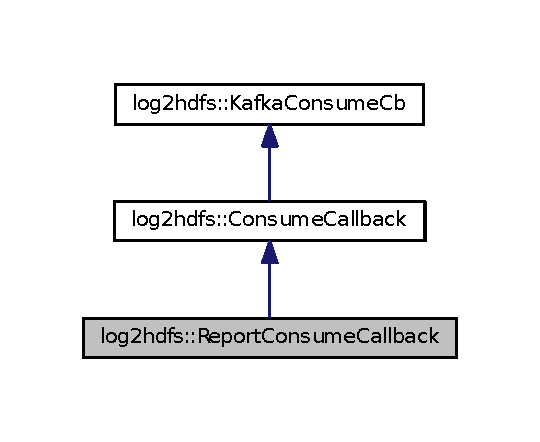
\includegraphics[width=259pt]{classlog2hdfs_1_1ReportConsumeCallback__inherit__graph}
\end{center}
\end{figure}


Collaboration diagram for log2hdfs\+:\+:Report\+Consume\+Callback\+:
\nopagebreak
\begin{figure}[H]
\begin{center}
\leavevmode
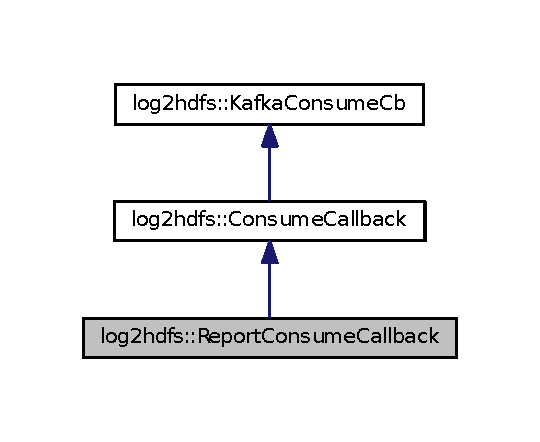
\includegraphics[width=259pt]{classlog2hdfs_1_1ReportConsumeCallback__coll__graph}
\end{center}
\end{figure}
\subsection*{Public Member Functions}
\begin{DoxyCompactItemize}
\item 
{\bfseries Report\+Consume\+Callback} (const std\+::string \&dir, std\+::shared\+\_\+ptr$<$ \hyperlink{classlog2hdfs_1_1PathFormat}{Path\+Format} $>$ format, std\+::shared\+\_\+ptr$<$ \hyperlink{classlog2hdfs_1_1FpCache}{Fp\+Cache} $>$ cache)\hypertarget{classlog2hdfs_1_1ReportConsumeCallback_ab97bc426819b659bdaaae4fddd6e5249}{}\label{classlog2hdfs_1_1ReportConsumeCallback_ab97bc426819b659bdaaae4fddd6e5249}

\item 
{\bfseries Report\+Consume\+Callback} (const \hyperlink{classlog2hdfs_1_1ReportConsumeCallback}{Report\+Consume\+Callback} \&other)=delete\hypertarget{classlog2hdfs_1_1ReportConsumeCallback_a7edcd4aa004d2a66209cfbfeb83de5e1}{}\label{classlog2hdfs_1_1ReportConsumeCallback_a7edcd4aa004d2a66209cfbfeb83de5e1}

\item 
\hyperlink{classlog2hdfs_1_1ReportConsumeCallback}{Report\+Consume\+Callback} \& {\bfseries operator=} (const \hyperlink{classlog2hdfs_1_1ReportConsumeCallback}{Report\+Consume\+Callback} \&other)=delete\hypertarget{classlog2hdfs_1_1ReportConsumeCallback_a0d11839ebab05d5e58a525226da584f6}{}\label{classlog2hdfs_1_1ReportConsumeCallback_a0d11839ebab05d5e58a525226da584f6}

\item 
void {\bfseries Consume} (const \hyperlink{classlog2hdfs_1_1KafkaMessage}{Kafka\+Message} \&msg)\hypertarget{classlog2hdfs_1_1ReportConsumeCallback_a926f5f60ba12cbfb3b80f1b78c9969ce}{}\label{classlog2hdfs_1_1ReportConsumeCallback_a926f5f60ba12cbfb3b80f1b78c9969ce}

\end{DoxyCompactItemize}
\subsection*{Static Public Member Functions}
\begin{DoxyCompactItemize}
\item 
static std\+::shared\+\_\+ptr$<$ \hyperlink{classlog2hdfs_1_1ReportConsumeCallback}{Report\+Consume\+Callback} $>$ {\bfseries Init} (std\+::shared\+\_\+ptr$<$ \hyperlink{classlog2hdfs_1_1TopicConf}{Topic\+Conf} $>$ conf, std\+::shared\+\_\+ptr$<$ \hyperlink{classlog2hdfs_1_1PathFormat}{Path\+Format} $>$ format, std\+::shared\+\_\+ptr$<$ \hyperlink{classlog2hdfs_1_1FpCache}{Fp\+Cache} $>$ cache)\hypertarget{classlog2hdfs_1_1ReportConsumeCallback_a95ecf78594436e916cadf6077823967f}{}\label{classlog2hdfs_1_1ReportConsumeCallback_a95ecf78594436e916cadf6077823967f}

\end{DoxyCompactItemize}
\subsection*{Additional Inherited Members}


The documentation for this class was generated from the following files\+:\begin{DoxyCompactItemize}
\item 
src/kafka2hdfs/consume\+\_\+callback.\+h\item 
src/kafka2hdfs/consume\+\_\+callback.\+cc\end{DoxyCompactItemize}

\hypertarget{classlog2hdfs_1_1Section}{}\section{log2hdfs\+:\+:Section Class Reference}
\label{classlog2hdfs_1_1Section}\index{log2hdfs\+::\+Section@{log2hdfs\+::\+Section}}
\subsection*{Public Types}
\begin{DoxyCompactItemize}
\item 
typedef std\+::unordered\+\_\+map$<$ std\+::string, std\+::string $>$\+::iterator {\bfseries iterator}\hypertarget{classlog2hdfs_1_1Section_a395082589cdd133dfed9f7880ba86e3c}{}\label{classlog2hdfs_1_1Section_a395082589cdd133dfed9f7880ba86e3c}

\item 
typedef std\+::unordered\+\_\+map$<$ std\+::string, std\+::string $>$\+::const\+\_\+iterator {\bfseries const\+\_\+iterator}\hypertarget{classlog2hdfs_1_1Section_af425058ae6ee4e199229dcdeaae1bda7}{}\label{classlog2hdfs_1_1Section_af425058ae6ee4e199229dcdeaae1bda7}

\end{DoxyCompactItemize}
\subsection*{Public Member Functions}
\begin{DoxyCompactItemize}
\item 
{\bfseries Section} (const \hyperlink{classlog2hdfs_1_1Section}{Section} \&other)\hypertarget{classlog2hdfs_1_1Section_adfaa5487e6313183cfb00f289a446278}{}\label{classlog2hdfs_1_1Section_adfaa5487e6313183cfb00f289a446278}

\item 
{\bfseries Section} (\hyperlink{classlog2hdfs_1_1Section}{Section} \&\&other)\hypertarget{classlog2hdfs_1_1Section_ab6e5e412a379873b636b2f0b9d51b7a9}{}\label{classlog2hdfs_1_1Section_ab6e5e412a379873b636b2f0b9d51b7a9}

\item 
\hyperlink{classlog2hdfs_1_1Section}{Section} \& {\bfseries operator=} (const \hyperlink{classlog2hdfs_1_1Section}{Section} \&other)\hypertarget{classlog2hdfs_1_1Section_ad9d6b66ff1ad2ffa7157ca7ff7a0e2c5}{}\label{classlog2hdfs_1_1Section_ad9d6b66ff1ad2ffa7157ca7ff7a0e2c5}

\item 
\hyperlink{classlog2hdfs_1_1Section}{Section} \& {\bfseries operator=} (\hyperlink{classlog2hdfs_1_1Section}{Section} \&\&other)\hypertarget{classlog2hdfs_1_1Section_a393bc4b0296173e4d2346f34ca9c0789}{}\label{classlog2hdfs_1_1Section_a393bc4b0296173e4d2346f34ca9c0789}

\item 
bool {\bfseries Has} (const std\+::string \&option) const \hypertarget{classlog2hdfs_1_1Section_a84000e3a5bcfd6e3b8ab219b038632e8}{}\label{classlog2hdfs_1_1Section_a84000e3a5bcfd6e3b8ab219b038632e8}

\item 
bool {\bfseries Remove} (const std\+::string \&option)\hypertarget{classlog2hdfs_1_1Section_aed0b35b429f51cd66f62d55153765be1}{}\label{classlog2hdfs_1_1Section_aed0b35b429f51cd66f62d55153765be1}

\item 
\hyperlink{classlog2hdfs_1_1Optional}{Optional}$<$ std\+::string $>$ {\bfseries Get} (const std\+::string \&option) const \hypertarget{classlog2hdfs_1_1Section_a5db65fc853dcde4963629a9117ccbb34}{}\label{classlog2hdfs_1_1Section_a5db65fc853dcde4963629a9117ccbb34}

\item 
std\+::string {\bfseries Get} (const std\+::string \&option, const std\+::string \&default\+\_\+value) const \hypertarget{classlog2hdfs_1_1Section_acd4eede29a5e80c7a5fefe759a49b9e1}{}\label{classlog2hdfs_1_1Section_acd4eede29a5e80c7a5fefe759a49b9e1}

\item 
bool {\bfseries Set} (const std\+::string \&option, const std\+::string \&value)\hypertarget{classlog2hdfs_1_1Section_ae87ec7d9f427d7960642e7ffce441320}{}\label{classlog2hdfs_1_1Section_ae87ec7d9f427d7960642e7ffce441320}

\item 
Section\+::iterator {\bfseries Begin} ()\hypertarget{classlog2hdfs_1_1Section_a53d856f5f884713c8a9af0a987f828db}{}\label{classlog2hdfs_1_1Section_a53d856f5f884713c8a9af0a987f828db}

\item 
Section\+::iterator {\bfseries End} ()\hypertarget{classlog2hdfs_1_1Section_aaf26649df0dfb29cfb183ca43bec1fc0}{}\label{classlog2hdfs_1_1Section_aaf26649df0dfb29cfb183ca43bec1fc0}

\item 
Section\+::const\+\_\+iterator {\bfseries Begin} () const \hypertarget{classlog2hdfs_1_1Section_aad7045f150705952a201a971674c3343}{}\label{classlog2hdfs_1_1Section_aad7045f150705952a201a971674c3343}

\item 
Section\+::const\+\_\+iterator {\bfseries End} () const \hypertarget{classlog2hdfs_1_1Section_a3460199936a5f723aa3576047c65e451}{}\label{classlog2hdfs_1_1Section_a3460199936a5f723aa3576047c65e451}

\item 
bool {\bfseries Empty} () const \hypertarget{classlog2hdfs_1_1Section_ae3d42af0cf5fd256b507c9e5a1e1c0d9}{}\label{classlog2hdfs_1_1Section_ae3d42af0cf5fd256b507c9e5a1e1c0d9}

\item 
void {\bfseries Clear} ()\hypertarget{classlog2hdfs_1_1Section_ae5a4b3417b3bd6e0aceaf50e481c3c9e}{}\label{classlog2hdfs_1_1Section_ae5a4b3417b3bd6e0aceaf50e481c3c9e}

\item 
bool {\bfseries Read} (const std\+::string \&filepath)\hypertarget{classlog2hdfs_1_1Section_a524b6063691869f2e2d1d353551386b5}{}\label{classlog2hdfs_1_1Section_a524b6063691869f2e2d1d353551386b5}

\item 
bool {\bfseries Write} (const std\+::string \&filepath) const \hypertarget{classlog2hdfs_1_1Section_a104102e5750e73b6fb6497f8561a2842}{}\label{classlog2hdfs_1_1Section_a104102e5750e73b6fb6497f8561a2842}

\item 
bool {\bfseries Write} (std\+::ofstream \&ofs) const \hypertarget{classlog2hdfs_1_1Section_ac478942a1456b7efed416ee5b65cec86}{}\label{classlog2hdfs_1_1Section_ac478942a1456b7efed416ee5b65cec86}

\end{DoxyCompactItemize}
\subsection*{Static Public Member Functions}
\begin{DoxyCompactItemize}
\item 
static std\+::shared\+\_\+ptr$<$ \hyperlink{classlog2hdfs_1_1Section}{Section} $>$ {\bfseries Init} ()\hypertarget{classlog2hdfs_1_1Section_ab0f923bf39efe934df970f2ca72ab65a}{}\label{classlog2hdfs_1_1Section_ab0f923bf39efe934df970f2ca72ab65a}

\end{DoxyCompactItemize}


The documentation for this class was generated from the following files\+:\begin{DoxyCompactItemize}
\item 
src/util/configparser.\+h\item 
src/util/configparser.\+cc\end{DoxyCompactItemize}

\hypertarget{classlog2hdfs_1_1TopicConf}{}\section{log2hdfs\+:\+:Topic\+Conf Class Reference}
\label{classlog2hdfs_1_1TopicConf}\index{log2hdfs\+::\+Topic\+Conf@{log2hdfs\+::\+Topic\+Conf}}
\subsection*{Public Member Functions}
\begin{DoxyCompactItemize}
\item 
{\bfseries Topic\+Conf} (const std\+::string \&section, const std\+::string \&rootdir)\hypertarget{classlog2hdfs_1_1TopicConf_a40be620420b87b5f1b80a6675c60beb2}{}\label{classlog2hdfs_1_1TopicConf_a40be620420b87b5f1b80a6675c60beb2}

\item 
bool {\bfseries Init\+Conf} (std\+::shared\+\_\+ptr$<$ \hyperlink{classlog2hdfs_1_1Section}{Section} $>$ section)\hypertarget{classlog2hdfs_1_1TopicConf_ae35b11051f7feb5203cf1f8d7efdbf89}{}\label{classlog2hdfs_1_1TopicConf_ae35b11051f7feb5203cf1f8d7efdbf89}

\item 
bool {\bfseries Update\+Runtime} (std\+::shared\+\_\+ptr$<$ \hyperlink{classlog2hdfs_1_1Section}{Section} $>$ section)\hypertarget{classlog2hdfs_1_1TopicConf_a7858567a96f4790bbb196576ca535e5e}{}\label{classlog2hdfs_1_1TopicConf_a7858567a96f4790bbb196576ca535e5e}

\item 
std\+::string {\bfseries consume\+\_\+dir} () const \hypertarget{classlog2hdfs_1_1TopicConf_a2cd48031f02615b895d479bf01c41ddc}{}\label{classlog2hdfs_1_1TopicConf_a2cd48031f02615b895d479bf01c41ddc}

\item 
std\+::string {\bfseries compress\+\_\+dir} () const \hypertarget{classlog2hdfs_1_1TopicConf_a3dc559a4cb24b275047983f2bc535ce3}{}\label{classlog2hdfs_1_1TopicConf_a3dc559a4cb24b275047983f2bc535ce3}

\item 
std\+::string {\bfseries upload\+\_\+dir} () const \hypertarget{classlog2hdfs_1_1TopicConf_ad2065d6901bd3f3401dce46389a744c4}{}\label{classlog2hdfs_1_1TopicConf_ad2065d6901bd3f3401dce46389a744c4}

\item 
{\bfseries Topic\+Conf} (const std\+::string \&topic)\hypertarget{classlog2hdfs_1_1TopicConf_ac99b8a0b746529f8141ad9121bc9dc97}{}\label{classlog2hdfs_1_1TopicConf_ac99b8a0b746529f8141ad9121bc9dc97}

\item 
bool {\bfseries Init\+Conf} (std\+::shared\+\_\+ptr$<$ \hyperlink{classlog2hdfs_1_1Section}{Section} $>$ section)\hypertarget{classlog2hdfs_1_1TopicConf_ae35b11051f7feb5203cf1f8d7efdbf89}{}\label{classlog2hdfs_1_1TopicConf_ae35b11051f7feb5203cf1f8d7efdbf89}

\item 
bool {\bfseries Update\+Runtime} (std\+::shared\+\_\+ptr$<$ \hyperlink{classlog2hdfs_1_1Section}{Section} $>$ section)\hypertarget{classlog2hdfs_1_1TopicConf_a7858567a96f4790bbb196576ca535e5e}{}\label{classlog2hdfs_1_1TopicConf_a7858567a96f4790bbb196576ca535e5e}

\item 
const std\+::string \& {\bfseries topic} () const \hypertarget{classlog2hdfs_1_1TopicConf_afd5c6e57b07373e2cf3f88e15b02323e}{}\label{classlog2hdfs_1_1TopicConf_afd5c6e57b07373e2cf3f88e15b02323e}

\item 
const std\+::vector$<$ std\+::string $>$ \& {\bfseries dirs} () const \hypertarget{classlog2hdfs_1_1TopicConf_ab7f1090d6a2fe326d016006fe5fe1dc1}{}\label{classlog2hdfs_1_1TopicConf_ab7f1090d6a2fe326d016006fe5fe1dc1}

\item 
std\+::unique\+\_\+ptr$<$ \hyperlink{classlog2hdfs_1_1KafkaTopicConf}{Kafka\+Topic\+Conf} $>$ {\bfseries kafka\+\_\+topic\+\_\+conf} () const \hypertarget{classlog2hdfs_1_1TopicConf_a91ba16c8d08aecd112729764bc1ad27f}{}\label{classlog2hdfs_1_1TopicConf_a91ba16c8d08aecd112729764bc1ad27f}

\item 
time\+\_\+t {\bfseries remedy} () const \hypertarget{classlog2hdfs_1_1TopicConf_a3f53ed29fd7bac2698de6c9b2fb6f0be}{}\label{classlog2hdfs_1_1TopicConf_a3f53ed29fd7bac2698de6c9b2fb6f0be}

\item 
int {\bfseries batch\+\_\+num} () const \hypertarget{classlog2hdfs_1_1TopicConf_acda3fad68a306cdfb0c2ccbfcd7d2eee}{}\label{classlog2hdfs_1_1TopicConf_acda3fad68a306cdfb0c2ccbfcd7d2eee}

\item 
int {\bfseries poll\+\_\+timeout} () const \hypertarget{classlog2hdfs_1_1TopicConf_a6240855dcfbe05164aec4d0167130e17}{}\label{classlog2hdfs_1_1TopicConf_a6240855dcfbe05164aec4d0167130e17}

\item 
int {\bfseries poll\+\_\+messages} () const \hypertarget{classlog2hdfs_1_1TopicConf_ad0cf4d98b1f9d3c7ec4d652f24697d86}{}\label{classlog2hdfs_1_1TopicConf_ad0cf4d98b1f9d3c7ec4d652f24697d86}

\end{DoxyCompactItemize}
\subsection*{Static Public Member Functions}
\begin{DoxyCompactItemize}
\item 
static bool {\bfseries Updata\+Default\+Conf} (std\+::shared\+\_\+ptr$<$ \hyperlink{classlog2hdfs_1_1Section}{Section} $>$ section)\hypertarget{classlog2hdfs_1_1TopicConf_a5180f284c0668f1345143bbb3f929f2f}{}\label{classlog2hdfs_1_1TopicConf_a5180f284c0668f1345143bbb3f929f2f}

\item 
static std\+::shared\+\_\+ptr$<$ \hyperlink{classlog2hdfs_1_1TopicConf}{Topic\+Conf} $>$ {\bfseries Init} (const std\+::string \&section, const std\+::string \&rootdir)\hypertarget{classlog2hdfs_1_1TopicConf_a55b5fe50959d06940eb8b4198eeef855}{}\label{classlog2hdfs_1_1TopicConf_a55b5fe50959d06940eb8b4198eeef855}

\item 
static bool {\bfseries Updata\+Default\+Conf} (std\+::shared\+\_\+ptr$<$ \hyperlink{classlog2hdfs_1_1Section}{Section} $>$ section)\hypertarget{classlog2hdfs_1_1TopicConf_aa022fa11f53f2edb7ed49dabce25cce9}{}\label{classlog2hdfs_1_1TopicConf_aa022fa11f53f2edb7ed49dabce25cce9}

\item 
static std\+::shared\+\_\+ptr$<$ \hyperlink{classlog2hdfs_1_1TopicConf}{Topic\+Conf} $>$ {\bfseries Init} (const std\+::string \&topic)\hypertarget{classlog2hdfs_1_1TopicConf_a095eb20dd881c8e261405934596ae3eb}{}\label{classlog2hdfs_1_1TopicConf_a095eb20dd881c8e261405934596ae3eb}

\end{DoxyCompactItemize}


The documentation for this class was generated from the following files\+:\begin{DoxyCompactItemize}
\item 
src/kafka2hdfs/topic\+\_\+conf.\+h\item 
src/log2kafka/topic\+\_\+conf.\+cc\end{DoxyCompactItemize}

\hypertarget{classlog2hdfs_1_1TopicConfContents}{}\section{log2hdfs\+:\+:Topic\+Conf\+Contents Class Reference}
\label{classlog2hdfs_1_1TopicConfContents}\index{log2hdfs\+::\+Topic\+Conf\+Contents@{log2hdfs\+::\+Topic\+Conf\+Contents}}
\subsection*{Friends}
\begin{DoxyCompactItemize}
\item 
class {\bfseries Topic\+Conf}\hypertarget{classlog2hdfs_1_1TopicConfContents_a432de442344920ee94b6271ab4996c39}{}\label{classlog2hdfs_1_1TopicConfContents_a432de442344920ee94b6271ab4996c39}

\end{DoxyCompactItemize}


The documentation for this class was generated from the following files\+:\begin{DoxyCompactItemize}
\item 
src/kafka2hdfs/topic\+\_\+conf.\+h\item 
src/log2kafka/topic\+\_\+conf.\+cc\end{DoxyCompactItemize}

\hypertarget{classlog2hdfs_1_1Upload}{}\section{log2hdfs\+:\+:Upload Class Reference}
\label{classlog2hdfs_1_1Upload}\index{log2hdfs\+::\+Upload@{log2hdfs\+::\+Upload}}
\subsection*{Public Types}
\begin{DoxyCompactItemize}
\item 
enum {\bfseries Type} \{ {\bfseries k\+None}, 
{\bfseries k\+Text}, 
{\bfseries k\+Lzo}, 
{\bfseries k\+Orc}
 \}\hypertarget{classlog2hdfs_1_1Upload_a383ff28c4a6efc47bf8588c49ee5f2ea}{}\label{classlog2hdfs_1_1Upload_a383ff28c4a6efc47bf8588c49ee5f2ea}

\end{DoxyCompactItemize}
\subsection*{Public Member Functions}
\begin{DoxyCompactItemize}
\item 
virtual bool {\bfseries Start} ()=0\hypertarget{classlog2hdfs_1_1Upload_a35ee440a177c814b2bb408447eab4d17}{}\label{classlog2hdfs_1_1Upload_a35ee440a177c814b2bb408447eab4d17}

\item 
virtual void {\bfseries Stop} ()=0\hypertarget{classlog2hdfs_1_1Upload_acc0649799b68b9883d6bdf792ccba1b2}{}\label{classlog2hdfs_1_1Upload_acc0649799b68b9883d6bdf792ccba1b2}

\end{DoxyCompactItemize}
\subsection*{Static Public Member Functions}
\begin{DoxyCompactItemize}
\item 
static std\+::unique\+\_\+ptr$<$ \hyperlink{classlog2hdfs_1_1Upload}{Upload} $>$ {\bfseries Init} (std\+::shared\+\_\+ptr$<$ \hyperlink{classlog2hdfs_1_1TopicConf}{Topic\+Conf} $>$ conf)\hypertarget{classlog2hdfs_1_1Upload_aad588f9de89484540b6a5b18bbd6be1c}{}\label{classlog2hdfs_1_1Upload_aad588f9de89484540b6a5b18bbd6be1c}

\end{DoxyCompactItemize}


The documentation for this class was generated from the following file\+:\begin{DoxyCompactItemize}
\item 
src/kafka2hdfs/upload.\+h\end{DoxyCompactItemize}

\hypertarget{classlog2hdfs_1_1V6ConsumeCallback}{}\section{log2hdfs\+:\+:V6\+Consume\+Callback Class Reference}
\label{classlog2hdfs_1_1V6ConsumeCallback}\index{log2hdfs\+::\+V6\+Consume\+Callback@{log2hdfs\+::\+V6\+Consume\+Callback}}


Inheritance diagram for log2hdfs\+:\+:V6\+Consume\+Callback\+:
\nopagebreak
\begin{figure}[H]
\begin{center}
\leavevmode
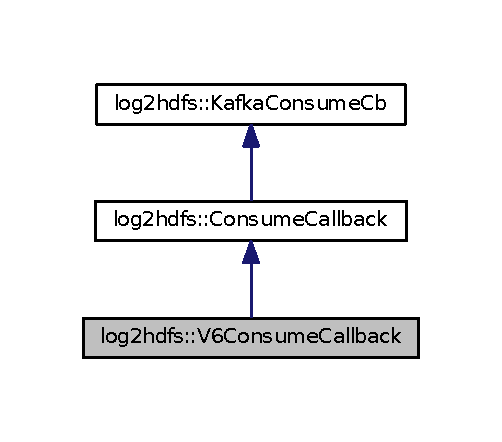
\includegraphics[width=241pt]{classlog2hdfs_1_1V6ConsumeCallback__inherit__graph}
\end{center}
\end{figure}


Collaboration diagram for log2hdfs\+:\+:V6\+Consume\+Callback\+:
\nopagebreak
\begin{figure}[H]
\begin{center}
\leavevmode
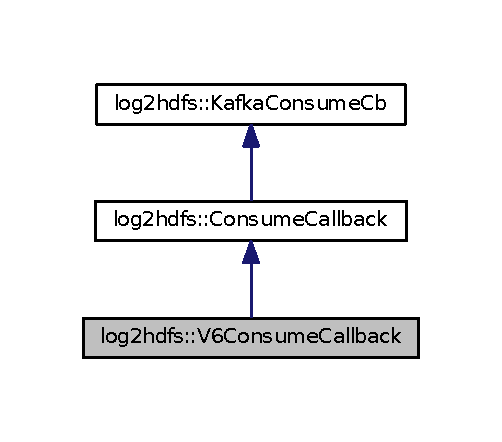
\includegraphics[width=241pt]{classlog2hdfs_1_1V6ConsumeCallback__coll__graph}
\end{center}
\end{figure}
\subsection*{Public Member Functions}
\begin{DoxyCompactItemize}
\item 
{\bfseries V6\+Consume\+Callback} (const std\+::string \&dir, std\+::shared\+\_\+ptr$<$ \hyperlink{classlog2hdfs_1_1PathFormat}{Path\+Format} $>$ format, std\+::shared\+\_\+ptr$<$ \hyperlink{classlog2hdfs_1_1FpCache}{Fp\+Cache} $>$ cache)\hypertarget{classlog2hdfs_1_1V6ConsumeCallback_a0318d8c237826367abfd58c4072095e5}{}\label{classlog2hdfs_1_1V6ConsumeCallback_a0318d8c237826367abfd58c4072095e5}

\item 
{\bfseries V6\+Consume\+Callback} (const \hyperlink{classlog2hdfs_1_1V6ConsumeCallback}{V6\+Consume\+Callback} \&other)=delete\hypertarget{classlog2hdfs_1_1V6ConsumeCallback_a1c2ee59c8f51913a55a76187b69ae911}{}\label{classlog2hdfs_1_1V6ConsumeCallback_a1c2ee59c8f51913a55a76187b69ae911}

\item 
\hyperlink{classlog2hdfs_1_1V6ConsumeCallback}{V6\+Consume\+Callback} \& {\bfseries operator=} (const \hyperlink{classlog2hdfs_1_1V6ConsumeCallback}{V6\+Consume\+Callback} \&other)=delete\hypertarget{classlog2hdfs_1_1V6ConsumeCallback_a19c034ceeb896fe2c93ab289e335f8b6}{}\label{classlog2hdfs_1_1V6ConsumeCallback_a19c034ceeb896fe2c93ab289e335f8b6}

\item 
void {\bfseries Consume} (const \hyperlink{classlog2hdfs_1_1KafkaMessage}{Kafka\+Message} \&msg)\hypertarget{classlog2hdfs_1_1V6ConsumeCallback_a0eaef4b1a9d52ccff835e0a18f40dd51}{}\label{classlog2hdfs_1_1V6ConsumeCallback_a0eaef4b1a9d52ccff835e0a18f40dd51}

\end{DoxyCompactItemize}
\subsection*{Static Public Member Functions}
\begin{DoxyCompactItemize}
\item 
static std\+::shared\+\_\+ptr$<$ \hyperlink{classlog2hdfs_1_1V6ConsumeCallback}{V6\+Consume\+Callback} $>$ {\bfseries Init} (std\+::shared\+\_\+ptr$<$ \hyperlink{classlog2hdfs_1_1TopicConf}{Topic\+Conf} $>$ conf, std\+::shared\+\_\+ptr$<$ \hyperlink{classlog2hdfs_1_1PathFormat}{Path\+Format} $>$ format, std\+::shared\+\_\+ptr$<$ \hyperlink{classlog2hdfs_1_1FpCache}{Fp\+Cache} $>$ cache)\hypertarget{classlog2hdfs_1_1V6ConsumeCallback_ad7e83f4b00d16a683bc3f85202b2e3b4}{}\label{classlog2hdfs_1_1V6ConsumeCallback_ad7e83f4b00d16a683bc3f85202b2e3b4}

\end{DoxyCompactItemize}
\subsection*{Additional Inherited Members}


The documentation for this class was generated from the following files\+:\begin{DoxyCompactItemize}
\item 
src/kafka2hdfs/consume\+\_\+callback.\+h\item 
src/kafka2hdfs/consume\+\_\+callback.\+cc\end{DoxyCompactItemize}

%--- End generated contents ---

% Index
\backmatter
\newpage
\phantomsection
\clearemptydoublepage
\addcontentsline{toc}{chapter}{Index}
\printindex

\end{document}
